\documentclass{elsinta}
\usepackage{url}
\usepackage{array}
\usepackage{longtable}
\usepackage{tikz}
\usetikzlibrary{shapes.geometric, arrows.meta, positioning}
\usepackage{adjustbox}

% --- Memasukkan Data Dokumen Menggunakan Perintah Baru ---
\projectcode{EL3}
\documentname{\SystemDesignTitle}
\documenttitle{Teknik Elektro - Sistem Informasi Tugas Akhir}
\capstonetitle{Monitoring on Induction Motor In Real-Time: Vibration and Temperature}
\shortname{MONTREAL-VT} 
\documentnumber{TA2526.01.099}
\revisionnumber{03}
\publicationdate{22 September 2025}

\revdatefooter{03/10/2025}
% --- Memasukkan Data Halaman Pengesahan (Halaman 2) ---
\currentpage{2} % Halaman yang sedang dicetak

% Data Tim
\ketuatimnama{Mahasiswa 1}
\ketuatimnim{12345678}

\anggotanamaI{Mahasiswa 2}
\anggotanimI{12345678}

\anggotanamaII{Mahasiswa 3}
\anggotanimII{12345678}


% Data Dosen
\pembimbingInama{Dosen 1}
\pembimbingInip{12345678 123456 1 123}

\pembimbingIInama{Dosen 2}
\pembimbingIInip{12345678 123456 1 123}


% Tanggal Pengesahan
\approvaldate{22 September 2025}

\begin{document}

% Panggil perintah untuk membuat halaman sampul
\coverpage
% Pindah ke Halaman Baru
\newpage

% Membuat Halaman Pengesahan (Halaman 2)
% \approvalpage

% Lanjut ke halaman proposal
\newpage

% ======================================
% Bagian Konten Proposal Dimulai di Sini
% ======================================

% Mengatur ulang nomor halaman dan gaya halaman
\clearpage
\pagenumbering{arabic}
\setcounter{page}{1} 
\pagestyle{myfooter} % Ganti dari 'plain' ke 'myfooter'

% Atur margin standar (Opsional, jika Anda ingin margin isi berbeda dari sampul)
% \newgeometry{left=4cm, right=3cm, top=3cm, bottom=3cm} 
% Catatan: Perintah \newgeometry memerlukan paket 'geometry' yang sudah ada di cls.

\tableofcontents
\newpage
\section*{\docsumary}
% Document Summary dalam sebuah capstone document berfungsi sebagai ringkasan utama yang memberikan gambaran singkat namun menyeluruh mengenai proyek akhir yang dikerjakan. Bagian ini biasanya dibaca pertama kali oleh dosen pembimbing, penguji, atau pihak luar, sehingga harus mampu menyampaikan inti dari keseluruhan laporan tanpa perlu membuka bab lain. Fokusnya adalah menjelaskan latar belakang permasalahan, tujuan proyek, serta kontribusi yang diharapkan dari capstone tersebut terhadap bidang keilmuan atau penerapan nyata.

% Isi Document Summary umumnya meliputi penjelasan singkat tentang masalah yang diangkat, metode atau pendekatan yang digunakan, serta ringkasan hasil utama yang dicapai. Jika proyek berbentuk implementasi sistem atau prototipe, maka bisa dijelaskan secara ringkas fitur utama atau inovasi yang menjadi keunggulan. Bagian ini juga dapat menyinggung keterkaitan proyek dengan kebutuhan industri atau masyarakat, sehingga nilai praktisnya lebih menonjol.

% Selain itu, Document Summary sebaiknya memuat ringkasan manfaat proyek, tantangan utama yang dihadapi, serta rekomendasi pengembangan ke depan. Dengan begitu, pembaca yang hanya membaca bagian ini sudah bisa memahami konteks, pendekatan, dan hasil dari capstone tanpa harus membaca seluruh isi dokumen. Singkatnya, Document Summary dalam capstone document harus menjadi "etalase" yang ringkas, padat, dan menarik, sekaligus mencerminkan esensi dari keseluruhan karya.

\newpage

\section{\SystemSpecTitle}
Spesifikasi sistem ditetapkan sebagai acuan dalam proses
pengembangan sistem Monitoring On Induction Motor In Real-Time:
Vibration and Temperature (MONTREAL-VT). Hal ini dilakukan 
untuk memastikan bahwa sistem yang dikembangkan memenuhi kriteria
sistem yang baik. Spesifikasi dibagi menjadi spesifikasi fungsional
yang menjelaskan fungsi yang harus dimiliki sistem, dan spesifikasi
non-fungsional yang menjabarkan kualitas yang harus
dicapai oleh fungsi sistem tersebut.

% ==============================================================
\subsection{\FunctionalSpecTitle}
Spesifikasi fungsional mencakup kemampuan yang harus 
dimiliki oleh sistem agar memenuhi tujuan pemantauan 
kondisi motor serperti tercantum pada tabel \ref{tab:fungsional}.

\renewcommand{\arraystretch}{1.3}
\begin{longtable}{|p{1.5cm}|p{7cm}|p{5cm}|}
    \caption{Spesifikasi Fungsional Sistem} \label{tab:fungsional} \\
    \hline
    \textbf{Kode} & \textbf{Spesifikasi Fungsional} & \textbf{Tujuan} \\
    \hline
    \endfirsthead
    
    \multicolumn{3}{c}{\tablename\ \thetable\ -- \textit{lanjutan dari halaman sebelumnya}} \\
    \hline
    Kode & \textbf{Spesifikasi Fungsional} & \textbf{Tujuan} \\
    \hline
    \endhead
    
    \hline
    \multicolumn{3}{r}{\textit{bersambung ke halaman berikutnya}} \\
    \endfoot
    
    \hline
    \endlastfoot
    
    F01 
    & Mengukur parameter akselerasi getaran 
    & Vibration Analysis\\
    \hline

    F02 
    & Mengukur suhu housing motor
    & Deteksi panas berlebih
    
    Tren suhu\\
    \hline

    F03 
    & Mengukur arus motor 
    & Pemantauan kondisi 
    pembebanan dan arus \\
    \hline

    F04 & Mengukur kecepatan rotasi (RPM) & Deteksi 
    perubahan kecepatan dan slip \\
    \hline

    
    F05 & Mengkonversi sinyal analog sensor menjadi 
    digital & Akuisisi data \\
    \hline
    F06 & Menerapkan pengkondisian sinyal pada keluaran 
    sensor & Peningkatan kualitas sinyal \\
    \hline
    F07 & Time-stamp setiap pengukuran & Sinkronisasi 
    parameter \\
    \hline
    F08 & Mentransmisikan data menuju cloud/server 
    menggunakan Wi-Fi & Upload to cloud, cloud-computing,
    remote monitoring \\
    \hline
    F09 & Menyimpan riwayat pengukuran pada basis data
    serverless & Analisis data historis \\
    \hline
    F10 & Menerapkan FFT pada data getaran & Deteksi 
    kerusakan melalui data domain-frekuensi\\
    \hline
    F11 & Menghitung indikator getaran (RMS, Peak, 
    Peak-to-Peak, dsb) & Penilaian kondisi mekanis \\
    \hline
    F12 & Memprediksi kerusakan bagian motor berlandaskan
    signature getaran yang tercantum pada ISO 20816 dan 
    13373 & Klasifikasi kerusakan \\
    \hline
    F13 & Mengkalkulasikan Health Index Motor & Penilaian
    kesehatan motor secara keseluruhan \\
    \hline
    F14 & Mengklasifikasikan tingkat kesehatan motor & Penilaian kesehatan motor secara keseluruhan \\
    \hline
    F15 & Memberikan perkiraan kerusakan pada bagian motor & Informasi kerusakan bagian motor \\
    \hline
    F16 & Menampilkan data akuisisi real-time pada dashboard & Pemantauan melalui HMI \\
    \hline
    F17 & Menampilkan tren historis getaran, arus, suhu, dan RPM & Predictive Maintenance \\
    \hline
    F18 & Mengaktifkan alarm ketika parameter melebihi batas yang telah ditentukan & Peringatan awal \\
    \hline
    F19 & Mengaktifkan output proteksi (SSR) pada kondisi kritis & Mencegah kerusakan motor \\
    \hline
    F20 & Log event alarm & Rekam perawatan (maintenance) \\
    \hline
\end{longtable}

\subsubsection{Use Case Diagram}
% Gambar \ref{fig:use_case} menjelaskan mengenai interaksi operator dan sistem.

\begin{figure}[t!]
    \centering
    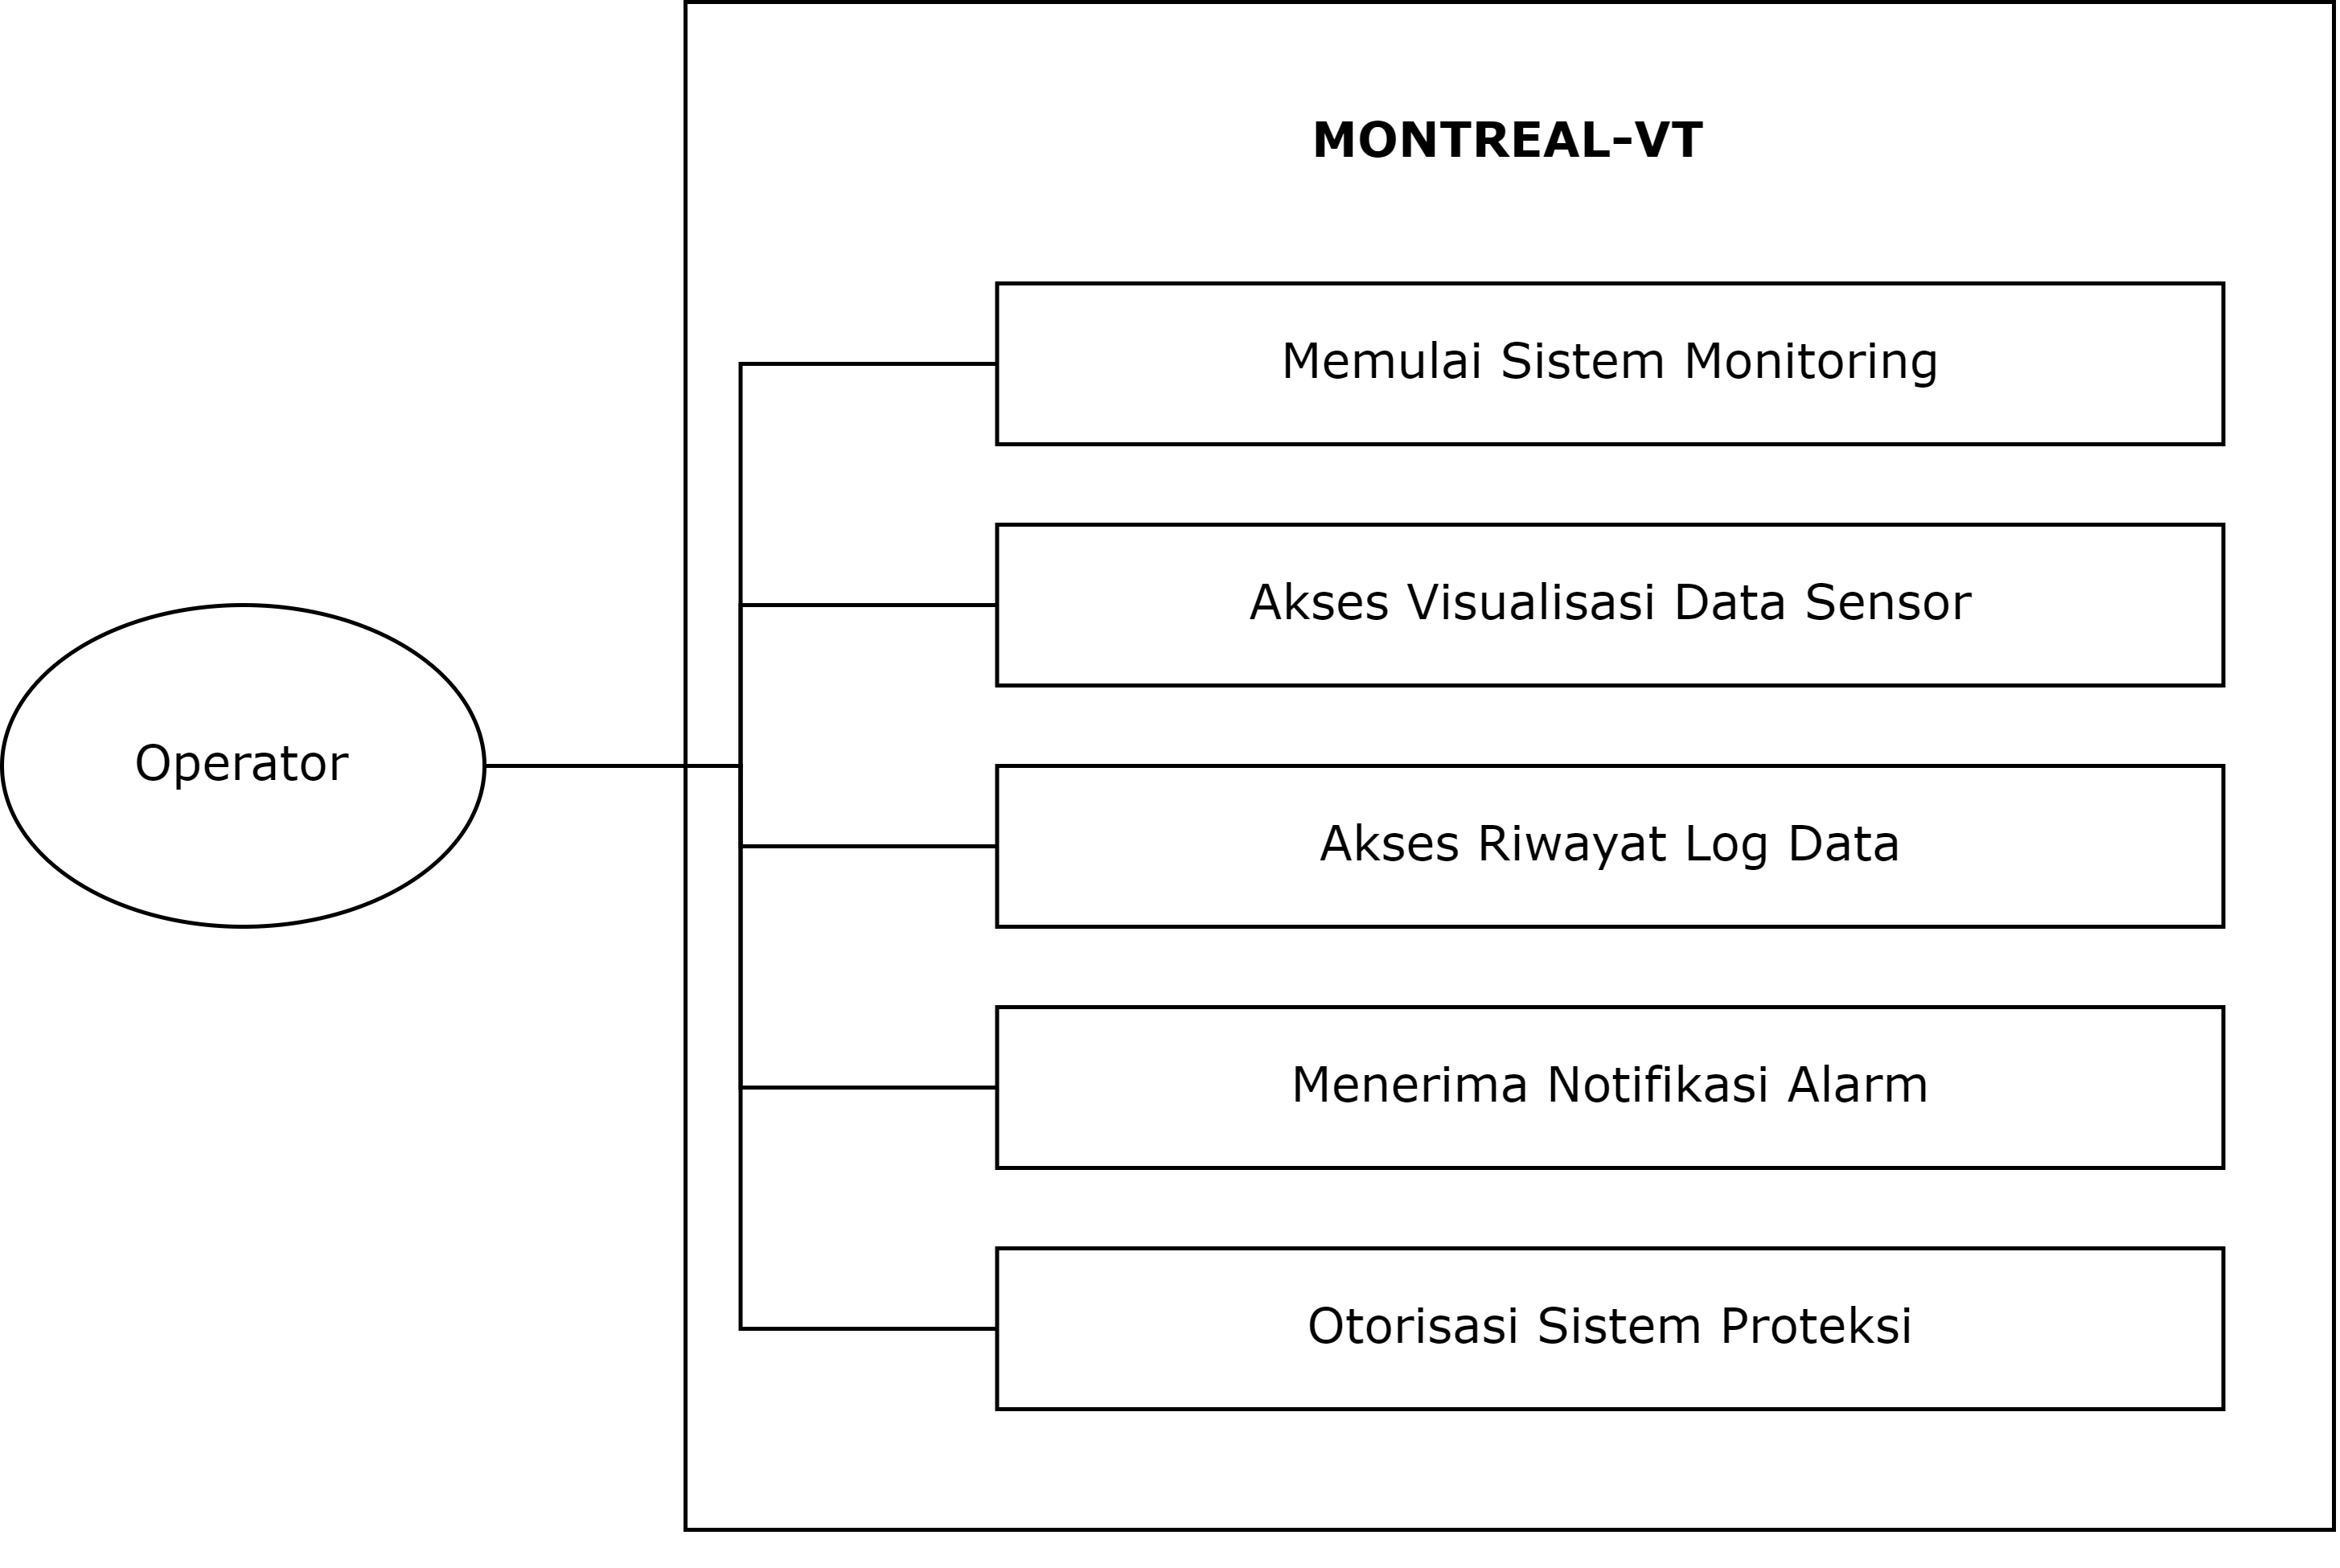
\includegraphics[width=0.8\textwidth]{image/doc/use_case_2.png} % Ganti dengan path diagram Anda
    \caption{Diagram Use Case MONTREAL-VT}
    \label{fig:use_case}
\end{figure}

% \subsubsection{Diagram Alir Sistem}
% Diagram alir menunjukkan cara kerja MONTREAL-VT dari inisialisasi sistem, proses akuisisi data, pemrograman sistem, hingga visualisasi dan notifikasi seperti pada gambar \ref{fig:flowchart} 

% \begin{figure}[H]
%     \centering
%     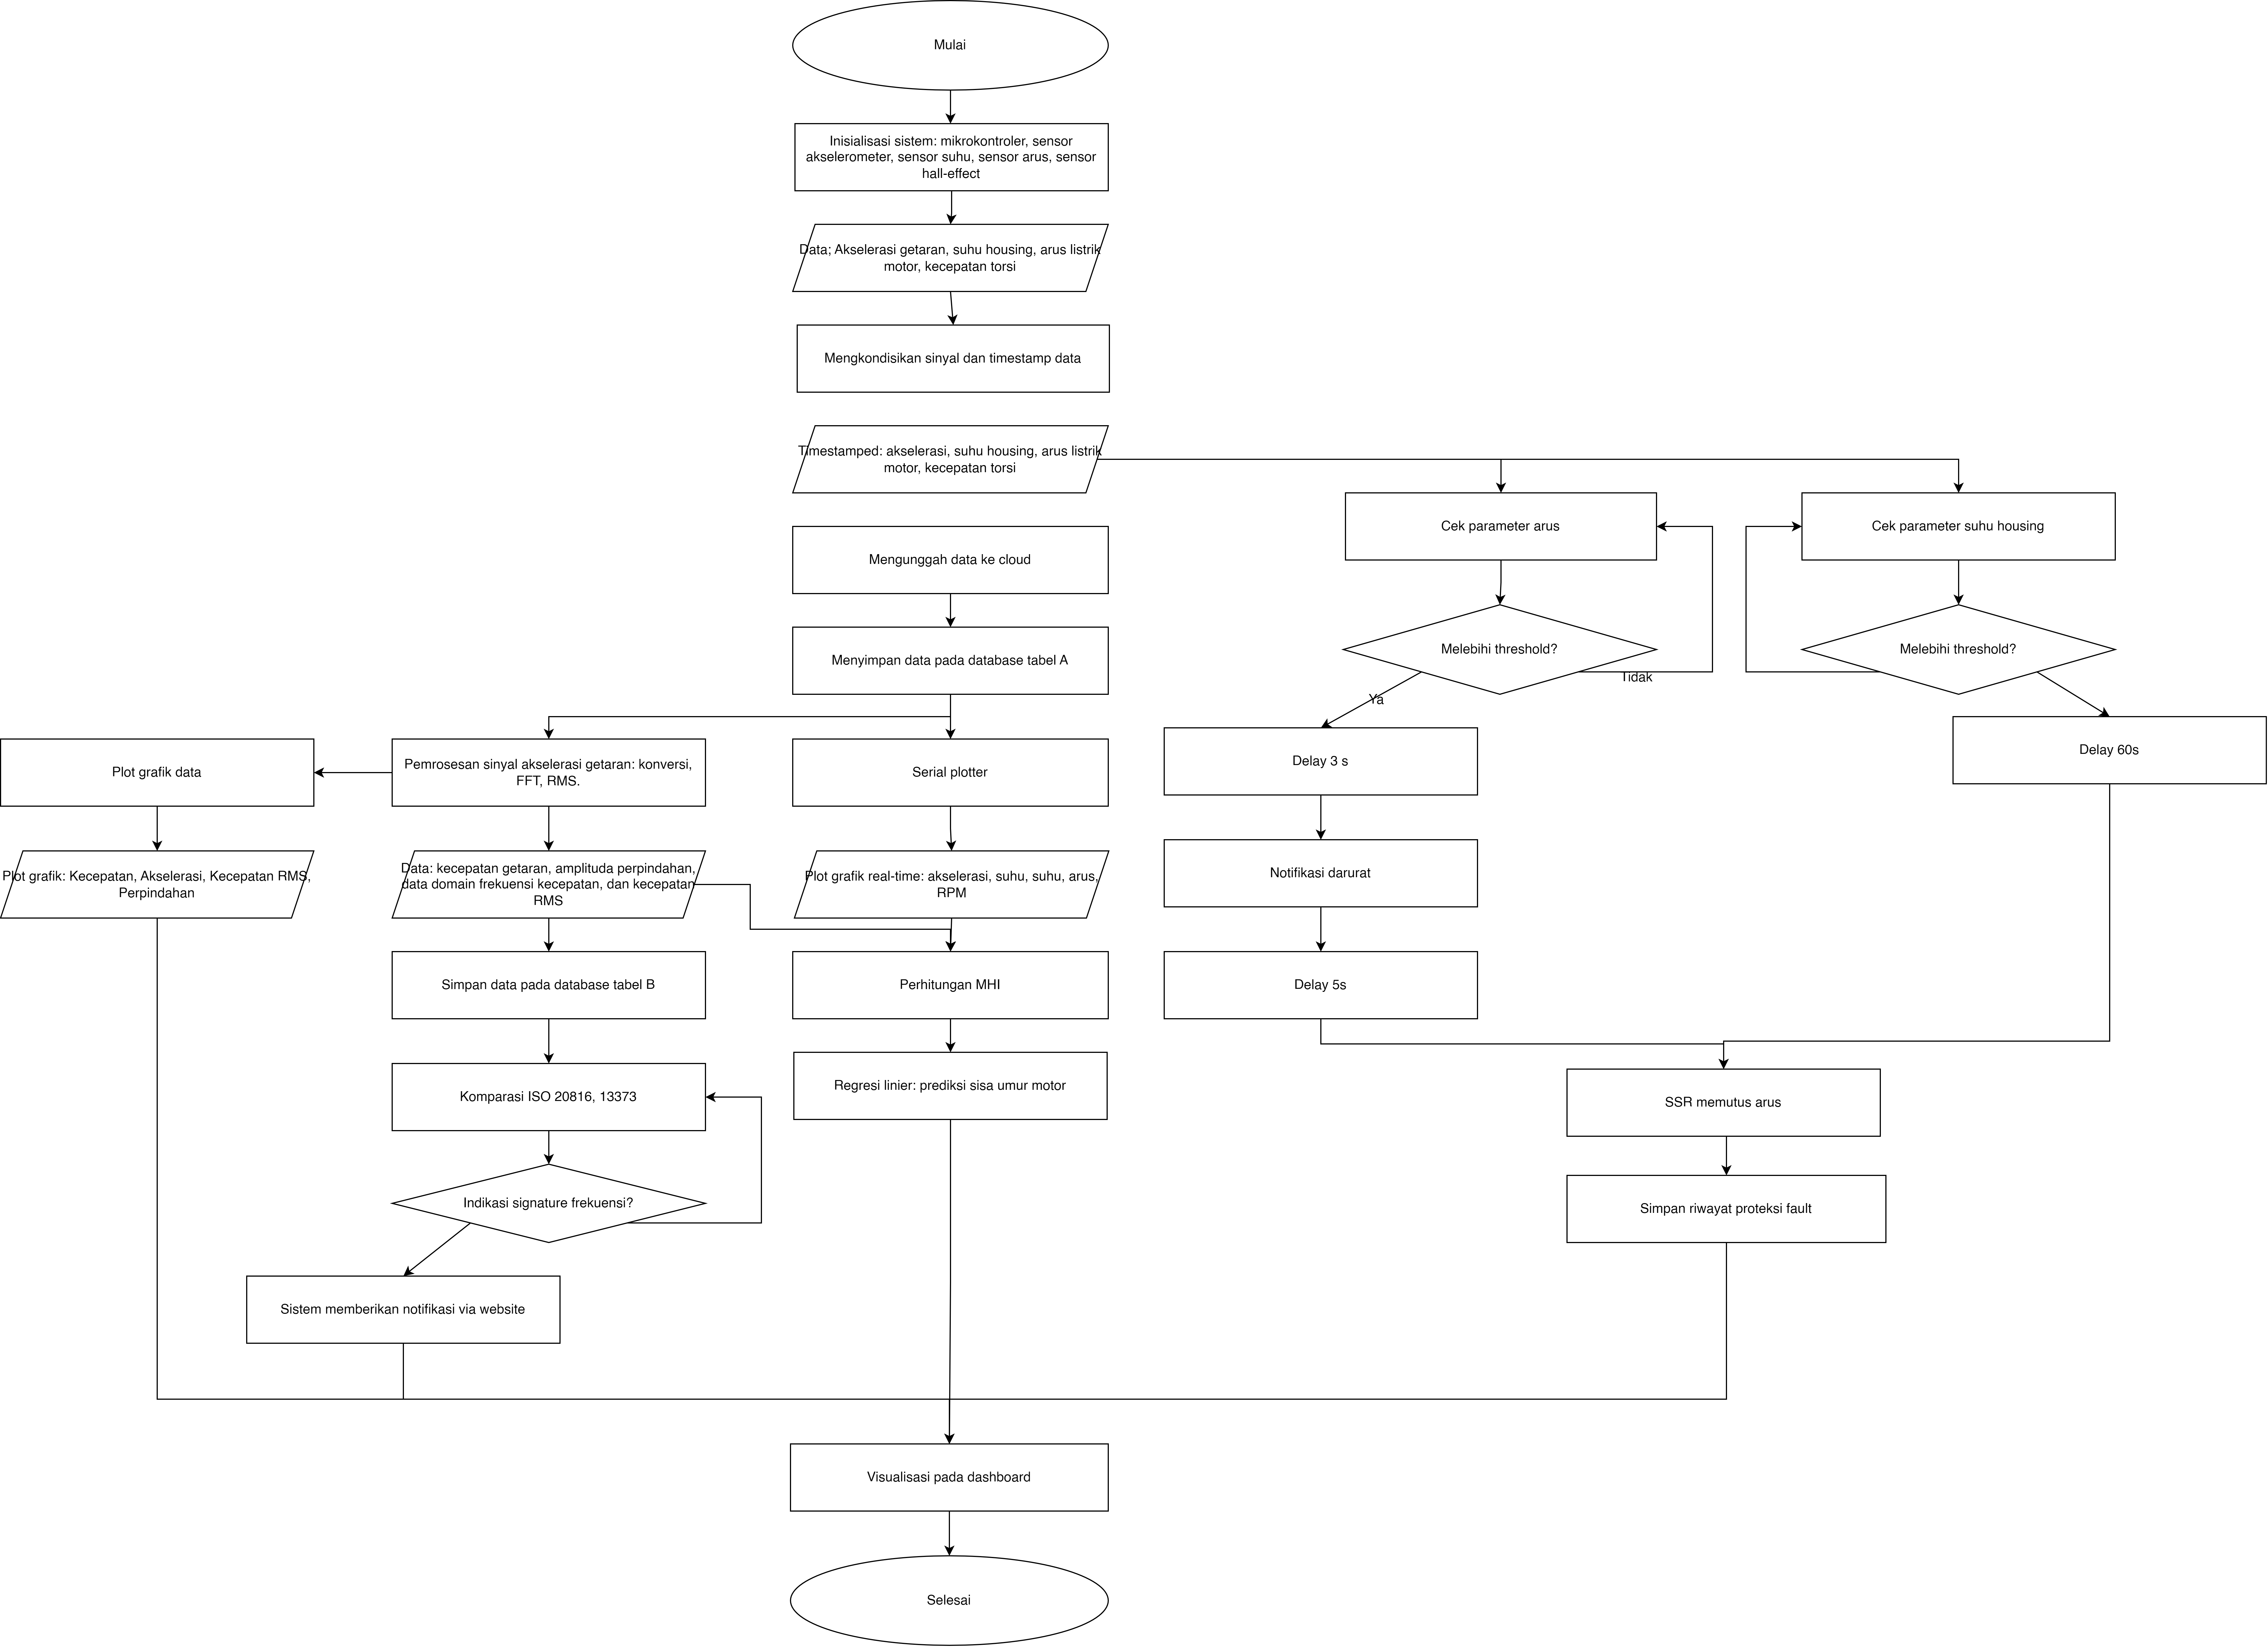
\includegraphics[width=\textwidth, height=0.7\textheight]{image/doc/flowchart_3.png}
%     \caption{Flowchart sistem MONTREAL-VT Opsi 1}
%     \label{fig:flowchart}
% \end{figure}

Desain kerja MONTREAL-VT dimulai dari inisialisasi 
komponen pada sistem, yakni mikrokontroler, sumber arus,
sensor, pengkondisian sinyal, dan komponen proteksi. 
Sensor mengukur data akselerasi getaran, 
suhu housing, arus listrik motor, dan kecepatan torsi, kumpulan data ini
tergolong sebagai data mentah. Data perolehan
sensor ini dikirimkan dalam bentuk sinyal yang akan 
dipre-proses pada proses pengkondisian sinyal baik pada
sistem pengkondisian analog ataupun digital pada mikrokontroler.

Lalu, sinyal yang telah dikondisikan akan dikonversi
menjadi data digital yang dikirimkan ke server cloud
dengan memanfaatkan modul Wi-Fi pada mikrokontroler.
Apabila tidak terdapat koneksi Wi-Fi, data akan disimpan
sementara pada memori eksternal (SD Card) hingga sistem
mendapatkan koneksi Wi-Fi. Data yang telah dikirimkan ke
server cloud disimpan pada basis data tabel A. Tabel A meliputi
data mentah yang telah dikondisikan.

Data tabel A akan diproses dalam 2 tahapan, yakni serial plotting
data mentah yang divisualisasikan secara real-time, dan pemrosesan sinyal akselerasi getaran
untuk mendapatkan indikator kecepatan getaran (cite ISO 13373).
Data kecepatan dan percepatan getaran akan digunakan untuk memprediksi
kerusakan bagian motor berdasarkan signature getaran yang tercantum pada
ISO 13373-1 lampiran C. Hasil pemrosesan lebih lanjut pada 
data getaran dikombinasikan dengan tren suhu, arus, dan RPM untuk
menghitung Indeks Kesehatan Motor (MHI) yang digunakan untuk
menilai tingkat kesehatan dan memprediksi sisa umur motor.

Selain sistem pemantauan, MONTREAL-VT dilengkapi dengan
sistem alarm dan proteksi. Sistem proteksi ini menggunakan
parameter ambang batas pada parameter arus dan suhu.




\subsection{\NonFunctionalSpecTitle}

%Perhitungan fmax dan Fs

% Spesifikasi non-fungsional menjelaskan karakteristik kualitas yang harus dipenuhi oleh sistem monitoring getaran dan suhu pada motor induksi. Selain mampu menjalankan fungsi utama, sistem juga harus memiliki kinerja yang baik, keandalan yang tinggi, keamanan, kemudahan penggunaan, serta kemampuan beroperasi secara stabil dalam proses monitoring kondisi motor. Karakteristik tersebut merupakan aspek penting dalam pengembangan sistem Internet of Things (IoT) yang menuntut kemampuan komunikasi data secara \textit{real-time}, andal, dan mudah diakses oleh pengguna \cite{bahga2014,mqtt311}.

\begin{longtable}{|p{1.5cm}|p{3cm}|p{9cm}|}
    \caption{Spesifikasi Non-Fungsional Sistem}
    \label{tab:nonfungsional} \\
    \hline
    \textbf{Kode} & \textbf{Aspek} & \textbf{Spesifikasi Non-Fungsional} \\
    \hline
    \endfirsthead

    \multicolumn{3}{c}{\tablename\ \thetable\ -- \textit{lanjutan dari halaman sebelumnya}} \\
    \hline
    \textbf{Kode} & \textbf{Aspek} & \textbf{Spesifikasi Non-Fungsional} \\
    \hline
    \endhead

    \hline
    \multicolumn{3}{r}{\textit{bersambung ke halaman berikutnya}} \\
    \endfoot

    \hline
    \endlastfoot

    NF01 & Pengukuran Getaran &
    Target bandwidth fault, $f_{max}=300Hz$

    $F_{s}=2 \times f_{max}=600Hz$
    
    \\
    \hline

    NF02 & Pengukuran Suhu &
    $F{s}=1Hz$
    
    Galat absolut,$\Delta=\pm 0.5^\circ C$, suhu ruang
    \\
    \hline

    NF03 & Frekuensi Pengukuran Arus &
    $F_{s}=1Hz$
    
     $\%error=4\%$    
    \\
    \hline

    NF04 & Pengukuran Kecepatan Putar (RPM) &
    $F_{s}=1400RPM/60s$
    $F_{s}=23.3Hz$
    \\
    \hline

    NF05 & MQTT &
    1s publish interval
    \\
    \hline

    NF06 & Dashboard &
    1s latency (maks)
    \\
    \hline

    NF07 & Interval pembaruan MHI &
    1s (maks)
    \\
    \hline

    NF08 &  Deteksi fault dan proteksi &
    3s delay (maks), sebelum notifikasi
    
    5s delay (maks), sebelum pemutusan arus
    \\
    \hline

    NF09 & Ketahanan Sistem &
    24 jam operasional
    \\
    \hline
    NF10 & FFT &
    1024 buffer size

    update latency 60s
    \\
    \hline
    
    NF10 & Koneksi &
    ESP32 reconnect otomatis ketika Wi-Fi terputus
    \\
    \hline
    
    NF11 & Autentikasi Dashboard &
    Dashboard hanya dapat diakses oleh otoritas yang diberi akses berupa password dan nomor ID.
    \\
    \hline

    NF12 & Kompatibilitas &
    Dashboard dapat diakses melalui browser PC, dan android.
    \\
    \hline

    NF13 & Maintanability &
    Software dikembangkan secara modular sehingga mudah dipelihara dan dikembangkan
    \\
    \hline

\end{longtable}


\subsubsection{Perhitungan Frekuensi Minimum Pengukuran Akselerasi Getaran}
    Spesifikasi motor yang digunakan adalah motor 
    induksi 1-fasa dengan kecepatan putar 1400 
    revolusi per menit;
    \[\omega=1400RPM\]
    \[\omega=\frac{1400}{60}\]
    \[\omega=23.3 Hz\]
    Maka satu revolusi penuh putaran kipas angin memiliki frekuensi $23.3 Hz$.
    
    Berdasarkan F12 pada tabel \ref{tab:fungsional}, sistem harus
    harus mampu memprediksi kerusakan bagian motor. Berdasarkan ISO 13373-1 lampiran C
    , pola getaran yang dihasilkan kerusakan meliputi $1\times$
    revolusi untuk unbalance dan misalignment, $2\times$ revolusi

    \[f_{fault}=300 Hz\]

    Maka dari itu, fmax pengukuran harus mampu menangkap detil
    dari frekuensi eksitasi yang mengindikasikan kerusakan.

    \[f_{max} \geq f_{fault}\] 
    \[f_{max} \geq 300 Hz\]

    Teori Nyquist-Shannon menyatakan bahwa frekuensi 
    sampling harus lebih besar dari dua kali 
    frekuensi sinyal yang diukur untuk menghindari terjadinya
    aliasing. Maka dari itu, frekuensi
    minimum pengukuran akselerasi getaran motor induksi
    adalah:

    \[F_{s} = 2 \cdot f_{max}\]
    \[F_{s} = 2 \cdot 300 Hz\]
    \[F_{s} = 600 Hz\]

\subsubsection{Perhitungan Batas Suhu Housing Maksimum}
    Berdasarkan panduan IEC 60034, pengukuran suhu motor dengan
    rating daya ($P_{rated} \leq 600W/VA$) (cite IEC 60034)
    harus dilakukan dengan metode termometer. 


\subsubsection{Perhitungan Batas Arus Motor Maksimum}
    Berdasarkan panduan IEC 60034, batas arus motor maksimum
    dapat ditentukan dari rating daya motor.
    \[P_{rated}=46W\] 
    \[P_{rated}=V_{rated} \cdot \eta \cdot cos(\Theta) \cdot I_{rated}\] 
    Persamaan dapat diubah
    \[I_{rated}=\frac{P_{rated}}{V_{rated} \cdot \eta \cdot \cos(\Theta)}\]

% Dari Tabel~\ref{tab:nonfungsional}, sistem tidak hanya dituntut mampu melakukan proses monitoring parameter motor induksi, tetapi juga harus memiliki kualitas layanan yang baik dari sisi kinerja, keandalan, keamanan, dan kemudahan penggunaan. Seluruh aspek tersebut menjadi acuan dalam proses implementasi dan pengujian sistem agar sistem yang dikembangkan memenuhi karakteristik perangkat IoT yang andal, mudah dipelihara, dan mampu beroperasi secara berkelanjutan \cite{bahga2014,PMBOK}.

% ==============================================================
\subsection{\HardwareSpecTitle}
% Spesifikasi perangkat keras menjelaskan komponen utama yang digunakan dalam perancangan sistem monitoring getaran dan suhu pada motor induksi. Perangkat keras terdiri atas sensor, mikrokontroler, modul komunikasi, aktuator, serta catu daya yang saling terintegrasi untuk memperoleh, mengolah, dan mengirimkan data kondisi motor secara \textit{real-time}. Pemilihan setiap komponen didasarkan pada kebutuhan sistem, kemudahan integrasi, serta kemampuan dalam mendukung proses monitoring dan proteksi motor induksi.

% Tabel \ref{tab:hardware} menunjukkan spesifikasi perangkat keras yang digunakan pada sistem.

\begin{longtable} {|p{1cm}|p{3cm}|p{3cm}|p{6cm}|}
    \caption{Spesifikasi Perangkat Keras}
    \label{tab:hardware-specs} \\
    \hline
    \textbf{No.} & \textbf{Komponen} & \textbf{Deskripsi} & \textbf{Spesifikasi Utama} \\
    \hline
    \endfirsthead

    \multicolumn{4}{c}{\tablename\ \thetable\ -- \textit{lanjutan dari halaman sebelumnya}} \\
    \hline
    \textbf{No.} & \textbf{Komponen} & \textbf{Deskripsi} & \textbf{Spesifikasi Utama} \\
    \hline
    \endhead

    \hline
    \multicolumn{4}{r}{\textit{bersambung ke halaman berikutnya}} \\
    \endfoot

    \hline\endlastfoot
    
    1 & 
    Capacitor-Starter SPIM (Model kipas angin Cosmos SN16) &
    Motor induksi 1-fasa &
    Kecepatan torsi 1400RPM
    
    Rating Daya 48W
    
    Tegangan 220VAC 50Hz
    
    Kapasitor 1.2uF \\
    \hline
    
    2 &
    ESP32-S3&
    Mikrokontroler utama &
    CPU Single/Dual-Core Xtensa 32-bit LX7 up to 240 MHz, ROM 384KB, SRAM 512KB, SRAM RTC 16KB
    
    IEEE 802.11b/g/n complied Wi-Fi 2.4 GHz band
    
    Bluetooth LE; Bluetooth 5, Bluetooth Mesh, Speed: 125Kbps/500Kbps/1Mbps/2Mbps
    
    45 GPIOs: 3 UART, 2 I2Cs, LCD interface, 2 general-purpose SPI ports, USB Serial/JTAG controller, SD/MMC host controller 2 slots, 2 Motor Control PWM (MCPWM), RMT (TX/RX), 2 12-bit SAR ADCs, up to 20 channels, temperature sensor, 4 54-bit general-purpose timers\\
    \hline
    
    3 & 
    ADXL345 &
    Sensor getaran motor &
    Sensor accelerometer 3-axis
    
    resolusi hingga 13-bit
    
    komunikasi I\textsuperscript{2}C/SPI
    
    rentang pengukuran ±2g hingga ±16g. \\
    \hline
    
    4 &
    DS18B20 &
    Sensor suhu motor &
    Rentang pengukuran -55$^\circ$C hingga 125$^\circ$C
    
    akurasi ±0.5$^\circ$C
    
    komunikasi One-Wire. \\
    \hline
    
    5 &
    ACS712 &
    Sensor arus motor &
    Sensor arus Hall Effect
    
    Rentang ±20 A
    
    tegangan kerja 5 V. \\
    \hline
    
    6 &
    Hall Effect Sensor &
    Sensor kecepatan putar motor (RPM) &
    Sensor digital berbasis efek Hall untuk mendeteksi jumlah putaran poros motor. \\
    \hline
    
    7 &
    Relay Module &
    Sistem proteksi motor &
    Relay 5 V
    
    kontak NO/NC
    
    kapasitas maksimum 10 A 250 VAC. \\
    \hline
    
    8 &
    Buzzer &
    Indikator alarm &
    Buzzer aktif 5 V sebagai indikator peringatan ketika kondisi motor abnormal. \\
    \hline
    
    9 &
    Power Supply &
    Catu daya sistem &
    Adaptor DC 5 V / 2 A untuk menyuplai seluruh perangkat elektronika. \\
    \hline
\end{longtable}

% ==============================================================
\subsection{\SoftwareSpecTitle}

% Perangkat lunak pada sistem monitoring getaran dan suhu motor induksi berfungsi untuk mengendalikan proses akuisisi data, pemrosesan sinyal, analisis kondisi motor, komunikasi data melalui jaringan Wi-Fi, serta visualisasi hasil monitoring pada dashboard. Arsitektur perangkat lunak dirancang secara modular sehingga setiap fungsi dapat dikembangkan dan dipelihara secara terpisah tanpa mempengaruhi fungsi lainnya \cite{bahga2014,ESP32}.

% Sistem perangkat lunak terdiri atas tiga lapisan utama, yaitu \textit{edge device}, \textit{cloud/server}, dan \textit{user interface}. Lapisan \textit{edge device} bertugas membaca data sensor, melakukan pemrosesan awal, dan mengirimkan data ke server. Lapisan \textit{cloud/server} berfungsi menyimpan data, mengelola data historis, serta menyediakan layanan komunikasi dengan dashboard. Sementara itu, lapisan \textit{user interface} berfungsi menampilkan hasil monitoring kepada pengguna secara \textit{real-time} melalui jaringan Internet \cite{bahga2014,mqtt311}.

% Tabel \ref{tab:software} menunjukkan spesifikasi perangkat lunak yang digunakan pada sistem monitoring motor induksi.

\begin{longtable}{|p{1cm}|p{4cm}|p{8.5cm}|}
\caption{Spesifikasi Perangkat Lunak}
\label{tab:software-specs}\\
\hline
\textbf{No.} & \textbf{Komponen} & \textbf{Spesifikasi} \\
\hline
\endfirsthead

\multicolumn{3}{c}{\tablename \thetable\ -- \textit{lanjutan dari halaman sebelumnya}} \\
\hline
\textbf{No.}& \textbf{Komponen} & \textbf{Spesifikasi} \\
\hline
\endhead

\hline
\multicolumn{3}{r}{\textit{bersambung ke halaman berikutnya}} \\
\endfoot

\hline\endlastfoot

1 & Bahasa Pemrograman &
C/C++, Python, JavaScript\\
\hline

2 & Framework &
Arduino Core ESP32 sebagai framework utama dalam pengembangan perangkat lunak mikrokontroler.\\
\hline

3 & Komunikasi Data &
Wi-Fi IEEE 802.11 b/g/n dengan protokol HTTP atau MQTT.\\
\hline

4 & Platform Cloud &
AWS IoT Core, Thingspeak.\\
\hline

5 & Database &
Macam
\\
\hline

6 & Dashboard Monitoring &
Dashboard berbasis Web atau Blynk IoT yang menampilkan parameter monitoring, grafik tren, status alarm, dan riwayat data.\\
\hline

7 & Pengolahan Data &
Perhitungan RMS, FFT, \textit{filtering} sinyal, serta penentuan kondisi motor berdasarkan nilai \textit{threshold}.\\
\hline

8 & Sistem Alarm &
Logika perangkat lunak untuk mengaktifkan buzzer dan relay apabila parameter melebihi batas operasi yang telah ditentukan.\\
\hline

9 & Data Logging &
Penyimpanan data monitoring yang dilengkapi informasi \textit{timestamp} untuk analisis historis.\\
\hline
\end{longtable}

% Dari Tabel~\ref{tab:software}, perangkat lunak pada ESP32 bertugas membaca data dari seluruh sensor, melakukan proses \textit{filtering}, menghitung parameter RMS dan FFT, kemudian menentukan kondisi motor berdasarkan nilai ambang (\textit{threshold}) yang telah ditetapkan. Selanjutnya, data dikirimkan melalui jaringan Wi-Fi menuju server sehingga dapat ditampilkan pada dashboard monitoring secara \textit{real-time}. Perangkat lunak juga mengendalikan sistem alarm dan relay proteksi apabila terdeteksi kondisi motor yang berada di luar batas operasi normal. Implementasi komunikasi IoT menggunakan protokol MQTT, sedangkan analisis sinyal getaran dilakukan menggunakan metode RMS dan Fast Fourier Transform (FFT) untuk memperoleh informasi kondisi motor secara akurat \cite{mqtt311,randall2011,oppenheim2010}.
% ==============================================================
\subsection{\PerformanceCriteriaTitle}

% Kriteria kinerja dan evaluasi diterapkan sebagai acuan untuk menilai keberhasilan sistem monitoring getaran dan suhu pada motor induksi yang dikembangkan. Pengujian dilakukan terhadap seluruh fungsi utama sistem, mulai dari akuisisi data sensor, pemrosesan sinyal, komunikasi data, visualisasi dashboard, hingga sistem alarm dan proteksi. Hasil pengujian ini akan dibandingkan dengan spesifikasi yang telah ditetapkan sehingga dapat diketahui tingkat keberhasilan implementasi sistem. Evaluasi kinerja merupakan tahapan penting dalam pengembangan sistem monitoring berbasis \textit{condition monitoring} dan \textit{predictive maintenance} untuk memastikan seluruh fungsi sistem bekerja sesuai dengan kebutuhan pengguna \cite{jardine2006,randall2011}.

Tabel \ref{tab:evaluasi} menunjukkan parameter yang digunakan sebagai acuan dalam pengujian sistem.

\begin{longtable}{|p{1cm}|p{5cm}|p{7cm}|}
\caption{Kriteria Kinerja dan Evaluasi Sistem}
\label{tab:evaluasi}\\
\hline
\textbf{No} & \textbf{Parameter Pengujian} & \textbf{Kriteria Keberhasilan} \\
\hline
\endfirsthead

\multicolumn{3}{c}{\tablename\ \thetable\ -- \textit{lanjutan dari halaman sebelumnya}} \\
\hline
\textbf{No} & \textbf{Parameter Pengujian} & \textbf{Kriteria Keberhasilan} \\
\hline
\endhead

\hline
\multicolumn{3}{r}{\textit{bersambung ke halaman berikutnya}} \\
\endfoot

\hline\endlastfoot

1 &
Sensor Getaran (ADXL345) &
Sensor mampu membaca data getaran secara stabil dan menghasilkan data sesuai kondisi operasi motor. \\
\hline

2 &
Sensor Suhu (DS18B20) &
Galat pengukuran suhu maksimum sebesar 15\% dibandingkan alat ukur referensi. \\
\hline

3 &
Sensor Arus (ACS712) &
Galat pengukuran arus maksimum sebesar 15\% dibandingkan alat ukur referensi. \\
\hline

4 &
Sensor Kecepatan (Hall Effect) &
Sensor mampu membaca kecepatan putar motor secara stabil selama pengujian. \\
\hline

5 &
Filtering Sinyal &
Proses filtering mampu mengurangi noise tanpa menghilangkan informasi utama pada sinyal. \\
\hline

6 &
Analisis RMS dan FFT &
Sistem mampu menghitung nilai RMS dan menampilkan spektrum frekuensi sinyal getaran. \\
\hline

7 &
Analisis Kondisi Motor &
Sistem mampu menentukan kondisi motor (Normal, Warning, atau Fault) berdasarkan nilai \textit{threshold} yang telah ditentukan. \\
\hline

8 &
Dashboard Monitoring &
Dashboard mampu menampilkan data sensor, grafik tren, serta status motor secara \textit{real-time}. \\
\hline

9 &
Komunikasi Data &
Data berhasil dikirim menuju dashboard dengan waktu tunda maksimum 1000 ms pada kondisi jaringan normal. \\
\hline

10 &
Alarm dan Proteksi &
Buzzer dan relay aktif ketika parameter monitoring melebihi batas operasi yang telah ditentukan. \\
\hline

11 &
Data Logging &
Data monitoring berhasil disimpan ke database lengkap dengan informasi \textit{timestamp}. \\
\hline

\end{longtable}

Berdasarkan Tabel~\ref{tab:evaluasi}, keberhasilan sistem tidak hanya ditentukan dari kemampuan membaca data sensor, tetapi juga kemampuan sistem dalam proses pengolahan sinyal, analisis kondisi motor, komunikasi data, visualisasi hasil monitoring, serta pemberian alarm dan proteksi ketika terjadi kondisi tidak normal. Pengujian terhadap parameter RMS dan Fast Fourier Transform (FFT) digunakan untuk mengevaluasi karakteristik getaran motor, sedangkan pengujian komunikasi data memastikan sistem mampu melakukan monitoring secara \textit{real-time} melalui jaringan Internet. Seluruh hasil pengujian tersebut menjadi dasar untuk menilai tingkat keandalan sistem monitoring yang dikembangkan \cite{oppenheim2010,randall2011,mqtt311}.

\section{\ProposedSolutionTitle}

% Bagian ini menyajikan gambaran menyeluruh tentang solusi yang diusulkan. Yang mencakup deskripsi produk/sistem secara umum, fitur-fitur kunci yang akan diimplementasikan, dan keunggulan kompetitif yang membedakannya dari solusi yang sudah ada.

% \textit{Penjelasan: Jelaskan secara naratif apa itu Project Tim Anda. Gambarkan secara singkat arsitektur sistem (misalnya, sensor, mikrokontroler, cloud, aktuator) dan bagaimana keseluruhan sistem bekerja. Tujuan utama adalah memberikan pemahaman yang jelas tentang konsep dan fungsionalitas inti proyek.}

\subsection{\ArchitectureTitle}
% \textit{Penjelasan: Bagian ini harus menguraikan arsitektur keseluruhan dari Project . Jelaskan bagaimana berbagai komponen (hardware, software, cloud) saling berinteraksi. Sangat disarankan untuk menyertakan diagram arsitektur sistem (Gambar ELx.y) yang memvisualisasikan subsistem-subsistem ini secara jelas. Kemudian, jelaskan setiap subsistem secara terperinci.}

% Arsitektur Project  dirancang secara modular untuk memastikan skalabilitas, kemudahan pengembangan, dan integrasi yang efisien antara komponen perangkat keras, perangkat lunak, dan layanan cloud. Arsitektur utama dibagi menjadi beberapa subsistem fungsional yang saling berinteraksi, membentuk sebuah solusi pemantauan dan pengendalian kualitas udara yang komprehensif. Seperti yang ditunjukkan pada Gambar \ref{fig:elsinta_arch}.

% \begin{tikzpicture}[
%     node distance=1.4cm and 1.8cm,
%     every node/.style={font=\sffamily\small},
%     box/.style={
%         rectangle, draw=black, thick, text width=3.6cm,
%         minimum height=1.4cm, align=center,
%         text=black, fill=white
%     },
%     ellip/.style={
%         ellipse, draw=black, thick, text width=3.2cm,
%         minimum height=1.6cm, align=center,
%         text=black, fill=white
%     },
%     arr/.style={-{Stealth[length=3mm]}, black, thick}
% ]

% % Nodes
% \node[ellip] (spim) {Capacitor-Starter SPIM};
% \node[box, below=of spim] (sensor) {Subsistem: Instalasi Sensor dan Pemrosesan Sinyal};
% \node[box, below left=1.6cm and 0.4cm of sensor] (komunikasi) {Subsistem: Komunikasi, Cloud, dan Algoritma};
% \node[box, below right=1.6cm and 0.4cm of sensor] (proteksi) {Subsistem: Desain Threshold dan Sistem Proteksi};

% % Arrows
% \draw[arr] (spim) -- (sensor);
% \draw[arr] (sensor.south) -- ++(0,-0.5) -| (komunikasi.north);
% \draw[arr] (sensor.south) -- ++(0,-0.5) -| (proteksi.north);
% \draw[arr] (proteksi.west) -- (komunikasi.east);

% % Feedback loop: proteksi -> spim
% \draw[arr] (proteksi.east) -- ++(1.5,0) |- (spim.east);

% \end{tikzpicture}

% --- Di sini Anda bisa menyisipkan Diagram Arsitektur Sistem ---
% Contoh:
\begin{figure}[b!]
    \centering
    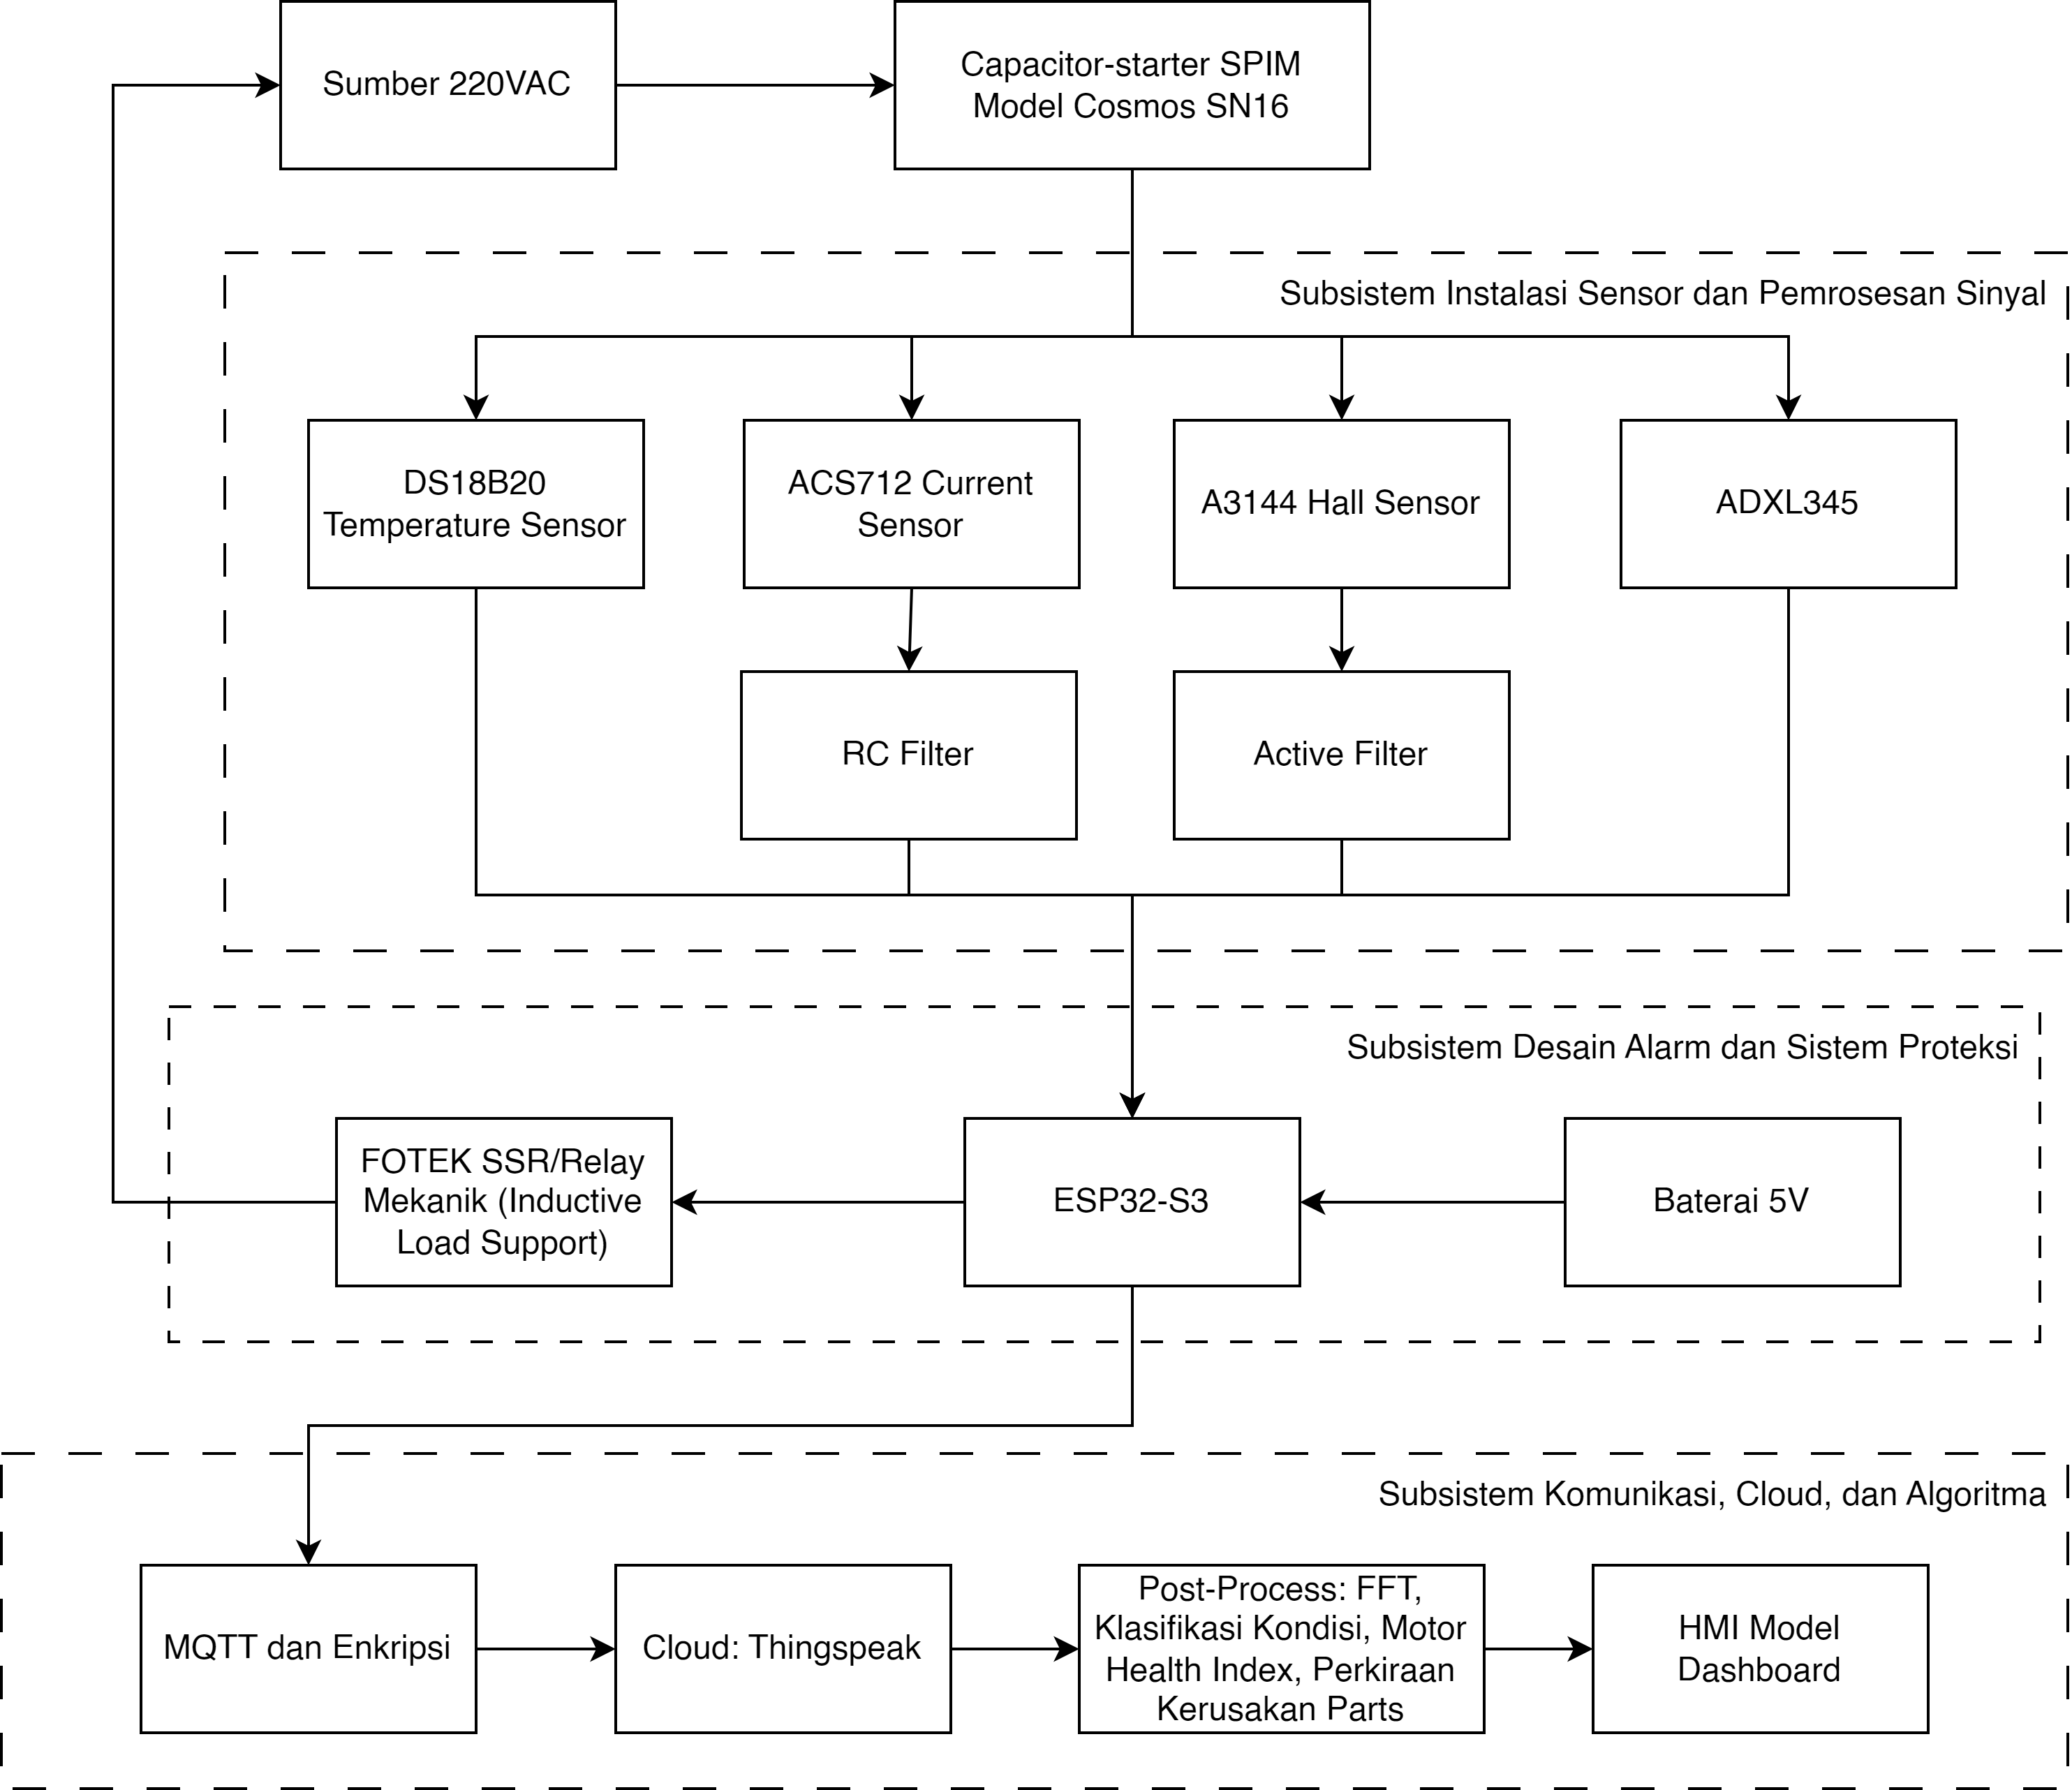
\includegraphics[width=0.8\textwidth]{image/doc/arsitektur_sistem_2.png} % Ganti dengan path diagram Anda
    \caption{Arsitektur Proyek}
    \label{fig:arsitektur}
\end{figure}

\textbf{MONTREAL-VT} merupakan sistem pemantauan motor induksi 1-fasa terintegrasi yang memiliki fitur dalam merekam, menyimpan, menganalisa data, dan memberikan informasi kepada operator mengenai kondisi motor. Parameter yang digunakan untuk menganalisa data meliputi getaran motor melalui sumbu x, y, dan z, suhu housing, arus motor, dan kecepatan putar motor.

Gambar \ref{fig:arsitektur} memaparkan arsitektur sistem MONTREAL-VT, terdiri atas tiga subsistem yang mencakup subsistem instalasi sensor dan pemrosesan sinyal, subsistem desain alarm dan sistem proteksi, dan sistem komunikasi, cloud, dan algoritma. 
% Ingat untuk menamai gambar Anda dengan format ELx.y yang sudah diatur.

\subsubsection{Subsistem Instalasi Sensor dan Pemrosesan Sinyal (ISPS)}
% \textit{Penjelasan: Fokus pada semua komponen fisik yang bertugas mengumpulkan data dari lingkungan. Sebutkan jenis sensor, mikrokontroler, dan modul-modul lain yang terlibat. Jelaskan bagaimana data dikumpulkan dan diproses secara lokal sebelum dikirim. }

\begin{figure}[H]
    \centering
    \includegraphics[width=0.8\textwidth]{image/doc/Flowchart-Page-1.png} % Ganti dengan path diagram Anda
    \caption{Flowchart Subsistem Instalasi Sensor dan Pemrosesan Sinyal (ISPS)}
    \label{fig:flowchart_isps}
\end{figure}

Instalasi Sensor dan Pemrosesan Sinyal (ISPS) merupakan 
subsistem yang mencakup proses pemilihan
 sensor dan instalasi yang sensor tepat,
  dan proses pengkondisian sinyal output
   dari sensor yang meliputi pemfilteran
    derau dan penguatan sinyal. 

Subsistem ini bertanggung jawab untuk instalasi, pengumpulan, dan pemrosesan sinyal output dari sensor getaran, sensor suhu, sensor arus, dan sensor RPM.
\begin{enumerate}
    \item \textbf{Kapasitor Starter SPIM:} Motor induksi satu fasa kipas angin model Cosmos 16SN, kecepatan putar 1400 RPM, 46W.
    \item \textbf{Unit Mikrokontroler:} Menggunakan $\text{ESP32}$. Mikrokontroler ini membaca data dari sensor, pra-pemrosesan, modul Wi-Fi, protokol komunikasi MQTT.
    \item \textbf{Modul Sensor Akselerometer ADXL345}: Modul sensor akselerometer digital 3-sumbu (X,Y,Z) dengan rentang +-2g hingga +-16g melalui I2C/SPI, sample-rate pengukuran hingga 3600Hz.
    \item \textbf{Sensor Suhu DS18B20 dan Driver:} Sensor suhu digital One-Wire yang memiliki rentang pengukuran -55C hingga +125C dengan akurasi +-0.5C pada rentang kerja normal. Sensor memiliki keluaran digital sehingga tidak memerlukan rangkaian penguat atau ADC tambahan.
    \item \textbf{Sensor Arus ACS172:} ACS712 merupakan sensor arus berbasis efek Hall yang mampu mengukur arus AC maupun DC dengan keluaran berupa tegangan analog yang proporsional terhadap arus.
    \item \textbf{Sensor Hall A3144 dan Magnet:} Sensor Hall A3144 digunakan bersama magnet permanen untuk mengukur kecepatan putar (RPM) motor melalui pendeteksian setiap putaran poros.
    \item \textbf{Operational Amplifier:} Operational Amplifier (Op-Amp) digunakan pada rangkaian pengkondisi sinyal untuk memperkuat, membuffer, dan memfilter sinyal sensor sebelum diproses mikrokontroler. Kegunaannya adalah untuk meningkatkan SNR, mengurangi gangguanw frekuensi tinggi.
    \item \textbf{Kapasitor:} Kapasitor digunakan sebagai decoupling/bypass capacitor untuk mengurangi ripple tegangan serta meredam noise tinggi, filter RC.
    \item \textbf{Resistor:} Resistor berfungsi untuk membatasi arus, mengatur level tegangan, serta membentuk konfigurasi yang sesuai.
\end{enumerate}
% Data yang terkumpul dari sensor akan diproses dan difilter di mikrokontroler sebelum dikirim ke subsistem komunikasi.

%%=========================Contoh Kode List, dan Algoritma==================================%%
% Contoh  Penulisan Algoritma  di Latex seperti pada Algoritme \autoref{alg:contoh1}:

% \begin{algorithm}[H]
% \caption{Pembacaan Sensor Suhu dan LED Control}
% \label{alg:contoh1}
% \begin{algorithmic}[1]
% \STATE Inisialisasi pin sensor dan LED
% \WHILE{true}
%     \STATE Baca nilai suhu dari sensor
%     \IF{suhu > 30$^\circ$C}
%         \STATE Nyalakan LED
%     \ELSE
%         \STATE Matikan LED
%     \ENDIF
%     \STATE Tunggu 1 detik
% \ENDWHILE
% \end{algorithmic}
% \end{algorithm}

% Contoh Script di Latex seperti pada \autoref{lst:arduino}: 
% \begin{lstlisting}[caption={Contoh Kode Arduino}, label={lst:arduino}]
% int led = 13;
% int sensor = A0;

% void setup() {
%   pinMode(led, OUTPUT);
% }

% void loop() {
%   int suhu = analogRead(sensor);
%   if (suhu > 600) digitalWrite(led, HIGH);
%   else digitalWrite(led, LOW);
%   delay(1000);
% }

% \end{lstlisting}
%%==================Contoh Codelist, dan Algoritma================================%%

\subsubsection{Subsistem Komunikasi, Cloud, dan Algoritma (KCA)}
% \textit{Penjelasan: Fokus pada bagaimana data dikirim dari perangkat keras ke server/cloud dan bagaimana data tersebut disimpan serta diproses lebih lanjut. Sebutkan protokol komunikasi (\text{MQTT}), platform  cloud (\text{AWS IoT, Firebase, Thingspeak}), dan database.}

Subsistem Komunikasi, Cloud, dan Algoritma (KCA) bertugas menghubungkan perangkat keras dengan infrastruktur cloud melalui protokol MQTT dan metode enkripsi, KCA juga bertanggung jawab atas post-processing sinyal sensor agar dapat digunakan untuk menganalisa keadaan motor.
\begin{enumerate}
    \item \textbf{Modul Komunikasi Nirkabel:} ESP32-S3 telah dilengkapi oleh modul Wi-Fi untuk menyediakan konektivitas internet. Modul ini memungkinkan proses pengiriman data hasil pengukuran sensor ke platform cloud secara nirkabel.
    \item \textbf{Protokol Komunikasi \text{IoT}:} Message Queuing Telemetry Transport (MQTT) merupakan protokol komunikasi utama antara ESP32-S3 dan platform cloud. MQTT bersifat ringan, memiliki konsumsi bandwidth yang rendah, serta mendukung komunikasi real-time yang andal.
    \item \textbf{Platform \text{Cloud} \text{IoT}:} AWS IoT Core merupakan platform cloud yang bertugas menerima data sensor melalui protokol MQTT. AWS IoT Core berfungsi sebagai MQTT broker sekaligus mekanisme autentikasi perangkat, pengelolaan koneksi, serta integrasi layanan AWS untuk pemrosesan dan analisis data.
    \item \textbf{Basis Data (\text{Database}):} Data sensor yang diterima AWS IoT Core akan diteruskan dan disimpan pada layanan penyimpanan AWS, Amazon DynamoDB dan Amazon S3. Data ini digunakan untuk analisis historis, dan visualisasi.
    \item \textbf{\emph{Dashboard} Berbasis Web:} Dashboard berbasis web yang bertugas dalam memvisualisasikan data secara real-time, visualisasi data historis, konfigurasi sistem, dan sistem notifikasi kondisi motor dan alarm. Dashboard dikembangkan menggunakan React, serta terhubung dengan layanan AWS.
\end{enumerate}
Data di cloud kemudian dapat diakses oleh subsistem visualisasi dan kontrol dari mana saja.

\begin{figure}[H]
    \centering
    \includegraphics[width=0.7\textwidth]{image/doc/Flowchart-Part-1-Page-2.png} % Ganti dengan path diagram Anda
    \caption{Flowchart Subsistem Komunikasi, Cloud, dan Algoritma (KCA)}
    \label{fig:flowchart_kca}
\end{figure}

\begin{algorithm}[H]
\caption{Pembacaan Sensor Suhu dan LED Control}
\label{alg:contoh1}
\begin{algorithmic}[1]
\STATE Inisialisasi pin sensor dan LED
\WHILE{true}
    \STATE Baca nilai suhu dari sensor
    \IF{suhu > 30$^\circ$C}
        \STATE Nyalakan LED
    \ELSE
        \STATE Matikan LED
    \ENDIF
    \STATE Tunggu 1 detik
\ENDWHILE
\end{algorithmic}
\end{algorithm}

\subsubsection{Subsistem Desain Alarm dan Sistem Proteksi (DASP)}
Subsistem Desain Alarm dan Sistem Proteksi (DASP) memiliki sistem dalam merancang arus dan suhu batas pada kerja motor, mendesain alarm peringatan dalam bentuk buzzer, dan visualisasi pada website, serta mengaktifkan relay proteksi apabila parameter arus dan suhu melewati batas dalam jangka waktu yang ditentukan.

\begin{enumerate}
    \item \textbf{ESP32-S3:} Berfungsi sebagai pengendali utama (main controller) yang menerima data dari seluruh sensor, melakukan komunikasi dengan platform cloud melalui jaringan Wi-Fi, menerima hasil analisis kondisi motor, serta mengeksekusi logika proteksi. Mikrokontroler ini mengendalikan aktivasi relay SSR untuk memutus atau menghubungkan catu daya motor berdasarkan kondisi operasi yang terdeteksi.

    \item \textbf{FOTEK SSR 20A:} Solid State Relay (SSR) digunakan sebagai aktuator proteksi yang berfungsi menghubungkan atau memutus suplai daya 220 VAC menuju motor induksi. SSR dikendalikan oleh sinyal keluaran ESP32-S3 sehingga proses pemutusan daya dapat dilakukan secara otomatis ketika sistem mendeteksi kondisi abnormal, seperti temperatur berlebih, getaran tinggi, arus berlebih, atau nilai Motor Health Index (MHI) yang berada di bawah batas aman.

    \item \textbf{Sistem Notifikasi:} Berfungsi memberikan peringatan kepada pengguna ketika parameter pemantauan melewati ambang batas yang telah ditentukan. Notifikasi ditampilkan pada dashboard secara real-time dan dapat dikirim melalui email atau layanan pesan sehingga pengguna dapat segera melakukan inspeksi maupun tindakan pemeliharaan.

    \item \textbf{Sumber Arus 220 VAC:} Merupakan sumber tegangan utama yang menyuplai motor induksi satu fasa. Jalur catu daya ini dikendalikan melalui SSR sehingga suplai listrik ke motor dapat diputus secara otomatis ketika sistem proteksi diaktifkan.

    \item \textbf{Saklar Manual (AZ5):} Digunakan sebagai saklar mekanis untuk menghubungkan atau memutus suplai daya secara manual. Saklar ini berfungsi sebagai lapisan proteksi tambahan (manual override) ketika terjadi kegagalan sistem elektronik, proses perawatan (maintenance), maupun kondisi darurat yang memerlukan penghentian operasi motor secara langsung.
\end{enumerate}

\begin{figure}[H]
    \centering
    \includegraphics[width=0.7\textwidth]{image/doc/Flowchart-Page-3.png} % Ganti dengan path diagram Anda
    \caption{Flowchart Subsistem Desain Alarm dan Sistem Proteksi (DASP)}
    \label{fig:flowchart_dasp}
\end{figure}

\subsection{\MainFeaturesTitle}
% \textit{Penjelasan: Daftarkan fitur-fitur utama yang akan disediakan oleh Project anda. Gunakan poin-poin yang jelas dan spesifik. Fokus pada apa yang dapat dilakukan oleh sistem yang tim buat.}

% \textbf{Contoh:} Berikut adalah fitur-fitur kunci yang akan diimplementasikan dalam \textbf{Project ELSINTA}:

\begin{enumerate}
    \item \textbf{Sistem Pemantauan Kondisi Motor Multi-Sensor:} Integrasi sensor ADXL345, ACS712, A314, dan DS18B20.
    \item \textbf{Notifikasi Kondisi dan Informasi Perkiraan Kerusakan Motor:} Notifikasi otomatis melalui website desain HMI, dan informasi perkiraan jenis kerusakan motor.
    \item \textbf{Sistem Proteksi Otomatis:} Memutus kontak arus apabila parameter arus dan suhu melebihi batas yang telah ditentukan.
\end{enumerate}

\subsection{\AdvantagesTitle}
% Penjelasan: Di bagian ini, bandingkan Project anda dengan solusi eksisting yang Anda bahas di \textbf{State of the Art} dan \textbf{Gap Analysis}. Tekankan mengapa proyek Anda lebih baik, lebih inovatif, atau lebih relevan, dengan merujuk kembali ke "celah" yang berhasil Anda isi. Fokus pada nilai tambah yang ditawarkan.

%Contoh:  Project ELSINTA menawarkan beberapa keunggulan signifikan dibandingkan solusi pemantauan dan pengendalian kualitas udara yang sudah ada di pasaran atau prototipe penelitian terdahulu:
\begin{enumerate}
    \item \textbf{Solusi Holistik dan Terintegrasi dengan Biaya Efektif:} 
\end{enumerate}

\subsection{\AlternativeDesignTitle}

\subsection{\JustificationTitle}
% \textit{Bagian ini bertujuan untuk menjustifikasi pemilihan komponen arsitektur utama Project dengan menganalisis solusi-solusi atau komponen alternatif yang sempat dipertimbangkan. Untuk setiap alternatif, jelaskan kelemahan spesifiknya yang menyebabkan penolakan, sehingga memperkuat argumen bahwa solusi yang dipilih adalah yang paling optimal berdasarkan kriteria biaya, kinerja, dan kompleksitas.}

% \textbf{Contoh}: Selama tahap desain, beberapa solusi alternatif telah dipertimbangkan sebelum memutuskan untuk mengembangkan arsitektur \text{IoT} berbasis $\text{ESP32}$ dan $\text{MQTT}$. Alternatif-alternatif tersebut antara lain:

\subsubsection*{Alternatif 1: Mikrokontroler ESP32-S3, Cloud Computing}
\begin{enumerate}
    \item \textbf{Deskripsi:} Alih-alih menggunakan $\text{WiFi}$, data sensor akan dikirim menggunakan koneksi kabel $\text{RS485}$ ke unit pusat (Gateway) yang kemudian mengirimkan data ke cloud.
    \item \textbf{Alasan Penolakan:} Meskipun $\text{RS485}$ menawarkan keandalan tinggi dan kekebalan kebisingan yang baik (teknis), ini memerlukan instalasi kabel yang kompleks, mahal, dan tidak fleksibel, sehingga bertentangan dengan tujuan proyek untuk menciptakan solusi yang mudah dipasang (\textit{plug-and-play}) dan efektif biaya.
\end{enumerate}

\begin{figure}[H]
    \centering
    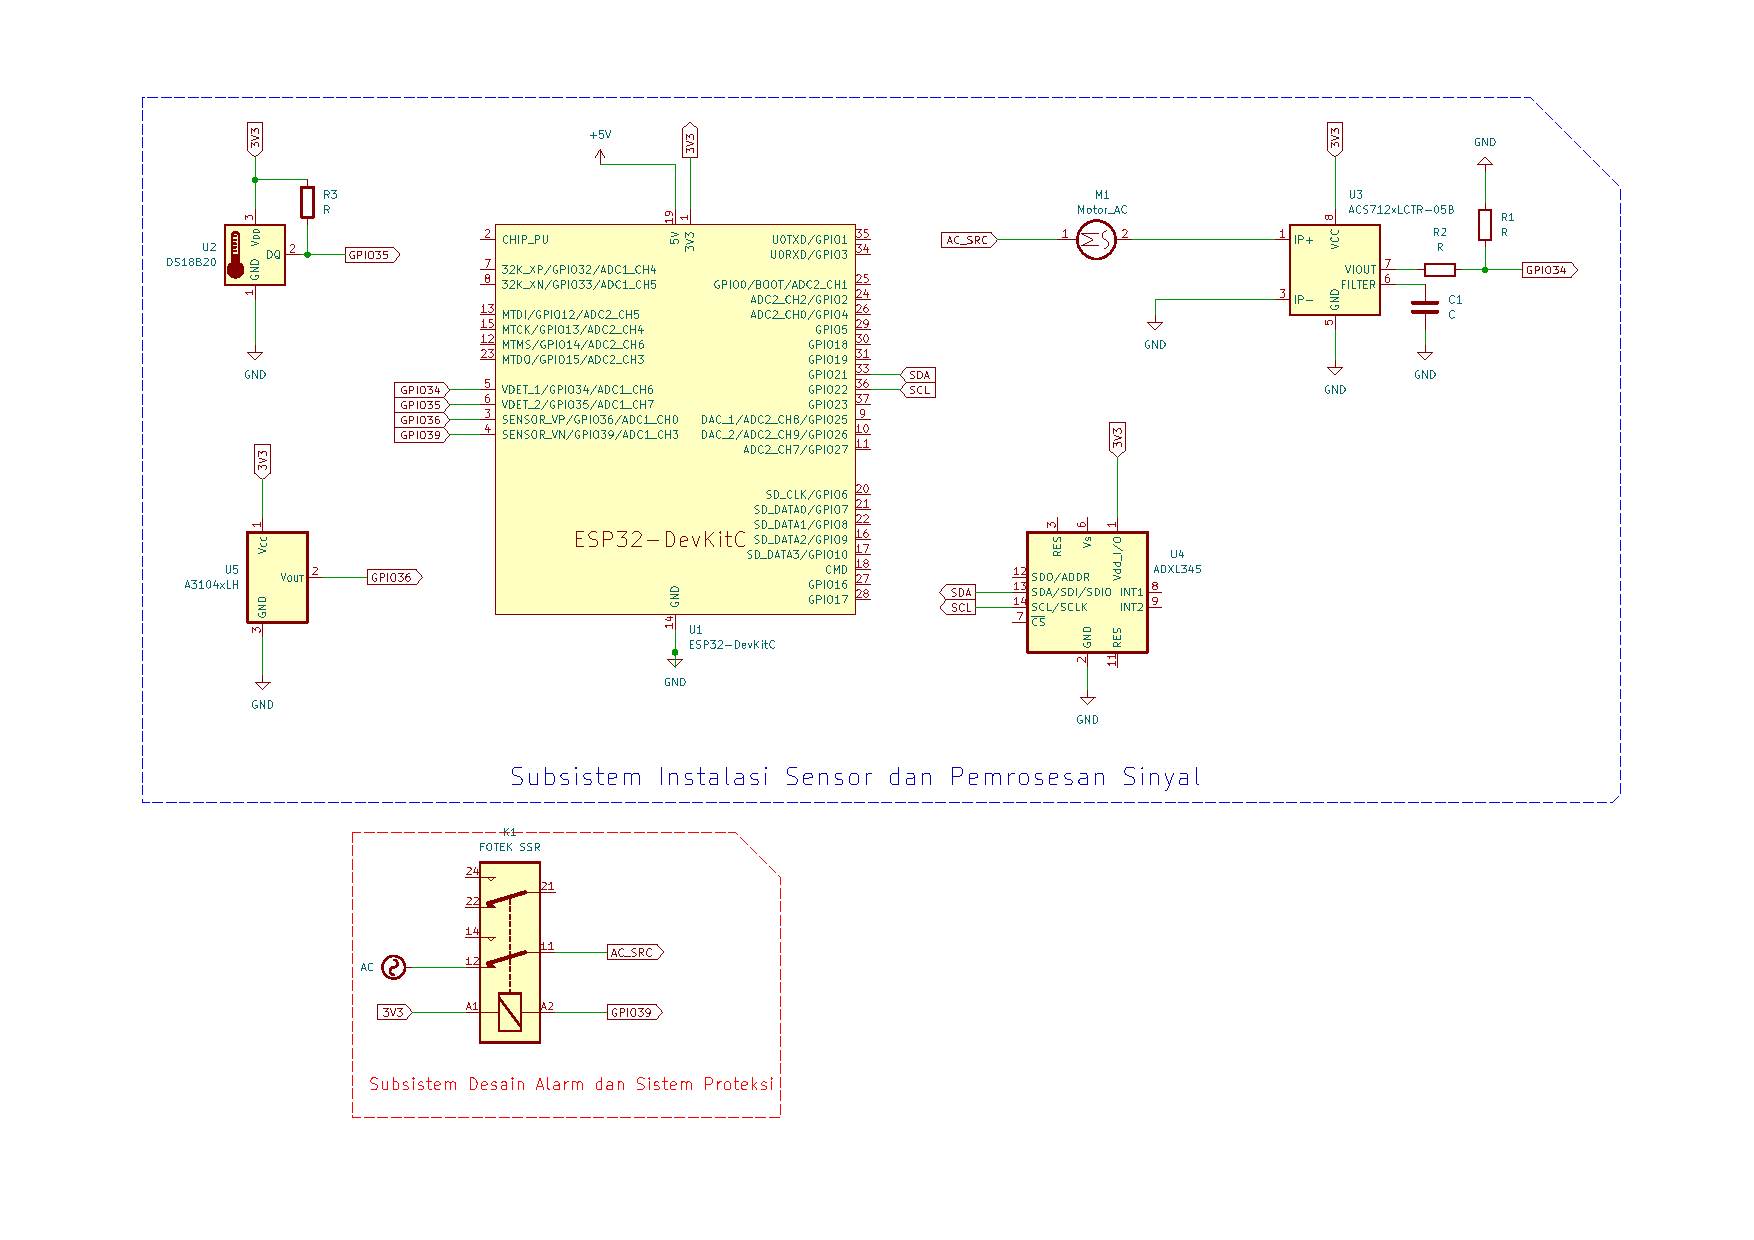
\includegraphics[width=0.8\textwidth]{image/doc/skematik-monitor.pdf} % Ganti dengan path diagram Anda
    \caption{Skematik desain alternatif 1}
    \label{fig:skematik}
\end{figure}

\subsubsection*{Alternatif 2: Raspberry Pi 4, Edge Computing}
\begin{enumerate}
    \item \textbf{Deskripsi:} Sistem hanya akan menggunakan mikrokontroler dan layar $\text{LCD}$ lokal untuk menampilkan data dan mengaktifkan alarm/kipas. Tidak ada koneksi internet, dashboard, atau penyimpanan data historis.
    \item \textbf{Alasan Penolakan:} Solusi ini tidak memenuhi kebutuhan kunci pasar akan akses data real-time dan analisis historis. Meskipun biayanya sangat rendah, kelemahan ini secara signifikan mengurangi dampak dan nilai tambah (\textit{value proposition}) proyek, terutama dalam konteks pelaporan dan manajemen risiko.
\end{enumerate}

\section{\ImplementationPlanTitle}

Work Breakdown Structure (WBS) merupakan dekomposisi pekerjaan proyek menjadi beberapa tahapan yang lebih terstruktur sehingga proses perancangan, implementasi, pengujian, dan dokumentasi dapat dilaksanakan secara sistematis. Penyusunan WBS bertujuan untuk mempermudah proses perencanaan, pengelolaan, serta pengawasan setiap aktivitas selama penelitian berlangsung.

Pada penelitian ini, WBS disusun berdasarkan tahapan pengembangan sistem \textit{Monitoring Getaran dan Suhu pada Motor Induksi}, mulai dari analisis kebutuhan sistem hingga penyusunan laporan akhir. Setiap tahapan memiliki keluaran (\textit{deliverable}) yang menjadi indikator keberhasilan sebelum melanjutkan ke tahap berikutnya.

\subsection{\WBSTitle}
% Work Breakdown Structure (WBS) merupakan metode dekomposisi pekerjaan proyek menjadi beberapa aktivitas yang lebih terstruktur sehingga memudahkan proses perencanaan, pengelolaan, pelaksanaan, dan evaluasi proyek. Penyusunan WBS pada penelitian ini disusun berdasarkan tahapan pengembangan sistem monitoring mulai dari analisis kebutuhan, perancangan, implementasi, pengujian, hingga dokumentasi akhir proyek sesuai praktik manajemen proyek \cite{PMBOK,kerzner2022}.

\textbf{WBS 1.1 Analisis Kebutuhan Sistem}

\textbf{Kegiatan:}
\begin{itemize}
    \item Mengidentifikasi kebutuhan sistem monitoring motor induksi.
    \item Menentukan parameter yang akan dimonitor, yaitu getaran, suhu, arus, dan kecepatan putar (RPM).
    \item Menyusun kebutuhan fungsional dan non-fungsional sistem.
\end{itemize}

\textbf{Deliverable:}
\begin{itemize}
    \item Dokumen kebutuhan sistem.
\end{itemize}

\textbf{WBS 1.2 Studi Literatur}

\textbf{Kegiatan:}
\begin{itemize}
    \item Studi mengenai motor induksi dan mekanisme kerusakannya \cite{nandi2005}.
    \item Studi karakteristik sensor ADXL345, DS18B20, ACS712, dan Hall Effect Sensor \cite{ADXL345,ACS712,A3144}.
    \item Studi metode pemrosesan sinyal seperti Filtering, RMS, dan FFT \cite{oppenheim2010,randall2011}.
    \item Studi sistem monitoring kondisi motor dan sistem proteksi \cite{jardine2006}.
\end{itemize}

\textbf{Deliverable:}
\begin{itemize}
    \item Dokumen studi literatur sebagai dasar perancangan sistem.
\end{itemize}

\textbf{WBS 1.3 Perancangan Arsitektur Sistem}

\textbf{Kegiatan:}
\begin{itemize}
    \item Menyusun diagram blok sistem.
    \item Menentukan arsitektur perangkat keras dan perangkat lunak.
    \item Menentukan pembagian subsistem sesuai pembagian tugas tim.
\end{itemize}

\textbf{Deliverable:}
\begin{itemize}
    \item Diagram blok sistem dan arsitektur sistem.
\end{itemize}

%====================================================
\subsubsection*{Fase 2 -- Perancangan Sistem (Minggu 3--5)}
%====================================================

\textbf{WBS 2.1 Perancangan Perangkat Keras}

\textbf{Kegiatan:}
\begin{itemize}
    \item Mendesain rangkaian ESP32.
    \item Mendesain rangkaian sensor getaran, suhu, arus, dan RPM.
    \item Mendesain sistem alarm dan proteksi.
\end{itemize}

\textbf{Deliverable:}
\begin{itemize}
    \item Skematik perangkat keras.
\end{itemize}

\textbf{WBS 2.2 Perancangan Perangkat Lunak}

\textbf{Kegiatan:}
\begin{itemize}
    \item Mendesain algoritma pembacaan sensor.
    \item Mendesain algoritma filtering sinyal.
    \item Mendesain algoritma RMS dan FFT \cite{oppenheim2010,randall2011}.
    \item Mendesain logika analisis kondisi motor.
\end{itemize}

\textbf{Deliverable:}
\begin{itemize}
    \item Flowchart perangkat lunak dan algoritma sistem.
\end{itemize}

\textbf{WBS 2.3 Perancangan Dashboard Monitoring}

\textbf{Kegiatan:}
\begin{itemize}
    \item Mendesain antarmuka dashboard monitoring.
    \item Mendesain struktur database.
    \item Mendesain sistem penyimpanan data (\textit{data logging}).
\end{itemize}

\textbf{Deliverable:}
\begin{itemize}
    \item Desain dashboard monitoring dan database.
\end{itemize}

%====================================================
\subsubsection*{Fase 3 -- Implementasi Sistem (Minggu 6--10)}
%====================================================

\textbf{WBS 3.1 Implementasi Subsistem Akuisisi Data dan Pemrosesan Sinyal}

\textbf{Kegiatan:}
\begin{itemize}
    \item Instalasi sensor pada motor induksi.
    \item Kalibrasi sensor.
    \item Akuisisi data getaran, suhu, arus, dan RPM.
    \item Implementasi filtering dan pengkondisian sinyal.
\end{itemize}

\textbf{Deliverable:}
\begin{itemize}
    \item Data sensor yang telah diproses dan siap dianalisis.
\end{itemize}

\textbf{WBS 3.2 Implementasi Subsistem Analisis Kondisi Motor}

\textbf{Kegiatan:}
\begin{itemize}
    \item Implementasi perhitungan RMS.
    \item Implementasi FFT.
    \item Analisis kondisi motor berdasarkan nilai \textit{threshold}.
   \item Implementasi dashboard monitoring.
\item Implementasi penyimpanan data (\textit{data logging}) menggunakan komunikasi IoT \cite{bahga2014,mqtt311}.
\end{itemize}

\textbf{Deliverable:}
\begin{itemize}
    \item Dashboard monitoring yang mampu menampilkan kondisi motor secara \textit{real-time}.
\end{itemize}

\textbf{WBS 3.3 Implementasi Subsistem Alarm dan Proteksi}

\textbf{Kegiatan:}
\begin{itemize}
    \item Implementasi sistem alarm.
    \item Implementasi relay proteksi.
    \item Implementasi \textit{event logging}.
    \item Pengujian fungsi alarm dan proteksi.
\end{itemize}

\textbf{Deliverable:}
\begin{itemize}
    \item Sistem alarm dan proteksi yang bekerja sesuai kondisi operasi motor.
\end{itemize}

%====================================================
\subsubsection*{Fase 4 -- Pengujian dan Validasi (Minggu 11--13)}
%====================================================

\textbf{WBS 4.1 Pengujian Perangkat Keras}

\begin{itemize}
    \item Pengujian fungsi seluruh sensor, ESP32, relay, dan buzzer.
\end{itemize}

\textbf{WBS 4.2 Pengujian Pemrosesan Sinyal}

\begin{itemize}
    \item Validasi hasil filtering, RMS, dan FFT terhadap data sensor.
\end{itemize}

\textbf{WBS 4.3 Pengujian Dashboard Monitoring}

\begin{itemize}
    \item Pengujian komunikasi data, visualisasi, dan penyimpanan data.
\end{itemize}

\textbf{WBS 4.4 Pengujian Alarm dan Proteksi}

\begin{itemize}
    \item Pengujian respon alarm dan relay terhadap kondisi abnormal.
\end{itemize}

\textbf{WBS 4.5 Pengujian Integrasi Sistem}

\begin{itemize}
    \item Pengujian keseluruhan sistem mulai dari pembacaan sensor hingga aktivasi alarm dan penyimpanan data.
\end{itemize}

\textbf{Deliverable:}
\begin{itemize}
    \item Laporan hasil pengujian dan validasi sistem.
    Tahap pengujian dilakukan untuk memastikan seluruh fungsi perangkat keras maupun perangkat lunak berjalan sesuai spesifikasi yang telah dirancang. Pengujian meliputi validasi sensor, analisis sinyal, komunikasi data, hingga pengujian integrasi sistem secara menyeluruh sehingga sistem memenuhi kebutuhan monitoring kondisi motor induksi \cite{PMBOK,jardine2006}.
\end{itemize}

%====================================================
\subsubsection*{Fase 5 -- Dokumentasi dan Pelaporan (Minggu 14--16)}
%====================================================

\textbf{WBS 5.1 Penyusunan Laporan Tugas Akhir}

\begin{itemize}
    \item Menyusun laporan hasil penelitian sesuai format Program Studi Teknik Elektro ITERA.
\end{itemize}

\textbf{WBS 5.2 Penyusunan Panduan Penggunaan Sistem}

\begin{itemize}
    \item Menyusun petunjuk instalasi, pengoperasian, dan pemeliharaan sistem monitoring.
\end{itemize}

\textbf{WBS 5.3 Persiapan Seminar Hasil}

\begin{itemize}
    \item Menyiapkan bahan presentasi, poster penelitian, dan demonstrasi sistem.
\end{itemize}

\textbf{Deliverable:}
\begin{itemize}
    \item Laporan tugas akhir.
    \item Buku panduan penggunaan sistem.
    \item Bahan presentasi seminar hasil.
\end{itemize}

\subsection{\TimelineTitle}
Jadwal implementasi disusun berdasarkan \textit{Work Breakdown Structure} (WBS) yang telah dijelaskan pada Subbab 3.1. Penyusunan jadwal bertujuan untuk mengatur urutan pelaksanaan setiap kegiatan sehingga proses pengembangan sistem dapat berlangsung secara sistematis dan sesuai target waktu yang telah ditetapkan. Seluruh aktivitas penelitian direncanakan berlangsung selama 16 minggu, dimulai dari tahap perencanaan hingga penyusunan laporan akhir. Setiap tahapan memiliki keterkaitan dengan tahapan sebelumnya sehingga penyelesaian suatu pekerjaan menjadi prasyarat untuk melanjutkan pekerjaan berikutnya.

Rencana jadwal implementasi penelitian ditunjukkan pada Tabel~\ref{tab:jadwal}.



\begin{table}[H]
\centering
\caption{Jadwal Implementasi Penelitian}
\label{tab:jadwal}
\renewcommand{\arraystretch}{1.3}
\begin{tabular}{|c|p{7cm}|c|c|c|}
\hline
No & Kegiatan & Minggu & Durasi & Ketergantungan\\
\hline

1 & Analisis kebutuhan sistem & 1--2 & 2 minggu & -\\
\hline

2 & Studi literatur & 1--2 & 2 minggu & -\\
\hline

3 & Perancangan arsitektur sistem & 2 & 1 minggu & 1,2\\
\hline

4 & Perancangan perangkat keras & 3--4 & 2 minggu & 3\\
\hline

5 & Perancangan perangkat lunak & 3--5 & 3 minggu & 3\\
\hline

6 & Perancangan dashboard monitoring & 4--5 & 2 minggu & 5\\
\hline

7 & Implementasi akuisisi data dan pemrosesan sinyal & 6--8 & 3 minggu & 4,5\\
\hline

8 & Implementasi analisis kondisi motor & 7--9 & 3 minggu & 7\\
\hline

9 & Implementasi alarm dan proteksi & 8--10 & 3 minggu & 7\\
\hline

10 & Pengujian perangkat keras & 11 & 1 minggu & 7\\
\hline

11 & Pengujian pemrosesan sinyal & 11--12 & 2 minggu & 8\\
\hline

12 & Pengujian dashboard monitoring & 12 & 1 minggu & 8\\
\hline

13 & Pengujian alarm dan proteksi & 12--13 & 2 minggu & 9\\
\hline

14 & Pengujian integrasi sistem & 13 & 1 minggu & 10--13\\
\hline

15 & Penyusunan laporan tugas akhir & 14--15 & 2 minggu & 14\\
\hline

16 & Penyusunan panduan penggunaan sistem & 15 & 1 minggu & 14\\
\hline

17 & Persiapan seminar hasil & 16 & 1 minggu & 15,16\\
\hline

\end{tabular}
\end{table}

\subsection{\TeamDivisionTitle}
Pembagian tugas tim dilakukan berdasarkan hasil diskusi bersama dosen pembimbing agar setiap anggota memiliki fokus penelitian yang berbeda sehingga tidak terjadi tumpang tindih dalam pengembangan sistem. Setiap anggota bertanggung jawab terhadap satu subsistem utama yang saling terintegrasi untuk membentuk sistem monitoring kondisi motor induksi secara menyeluruh.

Subsistem yang dikembangkan terdiri atas sistem instalasi sensor dan pemrosesan sinyal, sistem integrasi IoT dan algoritma klasifikasi kerusakan, serta sistem \textit{threshold} alarm dan proteksi. Pembagian tugas masing-masing anggota tim ditunjukkan pada Tabel~\ref{tab:pembagian_tugas}.

\begin{table}[H]
\centering
\caption{Pembagian Tugas Tim}
\label{tab:pembagian_tugas}

\renewcommand{\arraystretch}{1.4}

\begin{tabular}{|p{3cm}|p{4cm}|p{7cm}|}
\hline
\centering\textbf{Anggota Tim} &
\centering\textbf{Fokus Penelitian} &
\centering\arraybackslash\textbf{Tanggung Jawab}
\\
\hline

Mahasiswa A (Ketua Tim)
&
Instalasi Sensor dan Pemrosesan Sinyal
&
Instalasi sensor, kalibrasi sensor, akuisisi data, proses \textit{filtering}, penguatan sinyal (\textit{signal conditioning}), serta validasi hasil pengukuran sensor.
\\
\hline

Mahasiswa B
&
Integrasi IoT dan Algoritma Klasifikasi Kerusakan
&
Implementasi komunikasi IoT, pengolahan data menggunakan RMS dan FFT, \textit{data logging}, dashboard monitoring, \textit{Health Index}, klasifikasi kerusakan, dan estimasi \textit{breakdown}.
\\
\hline

Mahasiswa C
&
Threshold Alarm dan Sistem Proteksi
&
Penentuan nilai \textit{threshold}, implementasi alarm, relay proteksi, \textit{maintenance record}, \textit{event logging}, serta klasifikasi kategori gangguan (\textit{fault category}).
\\
\hline

\end{tabular}
\end{table}

Mahasiswa A bertanggung jawab terhadap pengembangan subsistem instalasi sensor dan pemrosesan sinyal. Ruang lingkup pekerjaan meliputi pemasangan sensor ADXL345, DS18B20, ACS712, dan Hall Effect Sensor pada motor induksi, proses kalibrasi sensor, akuisisi data, serta pengkondisian sinyal melalui proses \textit{filtering} dan penguatan sinyal. Luaran dari subsistem ini berupa data percepatan sumbu X, Y, dan Z, suhu motor, arus motor, tegangan AC, serta \textit{pulse count} yang siap digunakan untuk proses analisis.

Mahasiswa B bertanggung jawab terhadap pengembangan subsistem integrasi IoT dan algoritma klasifikasi kerusakan. Ruang lingkup pekerjaan meliputi implementasi komunikasi data melalui jaringan Wi-Fi, pengolahan sinyal menggunakan metode \textit{Root Mean Square} (RMS) dan \textit{Fast Fourier Transform} (FFT), penyimpanan data (\textit{data logging}), pencatatan \textit{timestamp}, visualisasi data melalui dashboard monitoring, klasifikasi kondisi motor, perhitungan \textit{Motor Health Index}, serta estimasi waktu menuju kondisi kritis (\textit{estimated breakdown}).

Mahasiswa C bertanggung jawab terhadap pengembangan subsistem \textit{threshold} alarm dan sistem proteksi. Ruang lingkup pekerjaan meliputi penentuan nilai ambang (\textit{threshold}), implementasi alarm, pengendalian relay proteksi, pencatatan \textit{maintenance record}, \textit{event logging}, serta klasifikasi kategori gangguan (\textit{fault category}). Subsistem ini berfungsi memberikan peringatan dini serta melakukan tindakan proteksi apabila parameter operasi motor melebihi batas yang telah ditentukan.

Ketiga subsistem tersebut dirancang agar saling terintegrasi. Subsistem instalasi sensor dan pemrosesan sinyal menghasilkan data hasil pengukuran yang selanjutnya diproses oleh subsistem integrasi IoT dan algoritma klasifikasi kerusakan. Hasil analisis kemudian digunakan oleh subsistem \textit{threshold} alarm dan sistem proteksi untuk menentukan status alarm serta tindakan proteksi sesuai kondisi operasi motor. Dengan pembagian tersebut, setiap anggota memiliki fokus penelitian yang berbeda namun tetap mendukung pengembangan sistem monitoring kondisi motor induksi secara menyeluruh.



\subsection{\SystemTestingTitle}


Pengujian sistem dilakukan untuk memverifikasi bahwa seluruh subsistem yang telah dirancang dapat berfungsi sesuai dengan spesifikasi fungsional dan non-fungsional yang telah ditetapkan. Pengujian ini bertujuan untuk memastikan bahwa proses akuisisi data, pengolahan sinyal, analisis kondisi motor, serta sistem alarm dan proteksi dapat bekerja secara terintegrasi dalam melakukan monitoring kondisi motor induksi.

Pengujian dilaksanakan secara bertahap yang meliputi pengujian masing-masing subsistem (\textit{unit testing}), pengujian integrasi (\textit{integration testing}), dan pengujian sistem secara keseluruhan (\textit{system testing}). Tahapan pengujian ini dilakukan untuk memastikan bahwa setiap subsistem mampu bekerja secara sinkron sehingga menghasilkan informasi kondisi motor yang akurat dan dapat digunakan sebagai dasar pengambilan keputusan pemeliharaan.

Parameter yang diuji meliputi akurasi pembacaan sensor, kualitas hasil pemrosesan sinyal, keberhasilan komunikasi data, kemampuan algoritma dalam mengidentifikasi kondisi motor, kecepatan respons alarm, serta fungsi sistem proteksi ketika terjadi kondisi abnormal.

Kriteria keberhasilan pengujian sistem ditunjukkan pada Tabel~\ref{tab:kriteria_pengujian}.

\begin{table}[H]
\centering
\caption{Kriteria Keberhasilan Pengujian Sistem}
\label{tab:kriteria_pengujian}
\renewcommand{\arraystretch}{1.3}

\begin{tabular}{|c|p{4.5cm}|p{4.2cm}|p{4cm}|}
\hline
\textbf{No} &
\centering\textbf{Parameter Pengujian} &
\centering\textbf{Metode Pengujian} &
\centering\arraybackslash\textbf{Kriteria Keberhasilan}\\
\hline

1 &
Akurasi sensor getaran (ADXL345) &
Dibandingkan dengan vibration meter &
Error $\leq$ 15\%\\
\hline

2 &
Akurasi sensor suhu (DS18B20) &
Dibandingkan dengan termometer digital &
Error $\leq$ 2$^\circ$C atau $\leq$ 5\%\\
\hline

3 &
Akurasi sensor arus (ACS712) &
Dibandingkan dengan clamp meter &
Error $\leq$ 10\%\\
\hline

4 &
Akurasi pembacaan RPM &
Dibandingkan dengan tachometer &
Error $\leq$ 5\%\\
\hline

5 &
Pengiriman data IoT &
Monitoring dashboard &
Keberhasilan pengiriman $\geq$ 98\%\\
\hline

6 &
Delay komunikasi data &
Pengukuran waktu pengiriman &
Delay $\leq$ 3 detik\\
\hline

7 &
Perhitungan RMS &
Dibandingkan dengan MATLAB/Python &
Error $\leq$ 5\%\\
\hline

8 &
Analisis FFT &
Dibandingkan dengan spektrum referensi &
Frekuensi dominan sesuai referensi\\
\hline

9 &
Klasifikasi kondisi motor &
Pengujian beberapa kondisi motor &
Akurasi klasifikasi $\geq$ 90\%\\
\hline

10 &
Motor Health Index &
Validasi terhadap kondisi motor &
Sesuai kondisi aktual motor\\
\hline

11 &
Alarm &
Simulasi melewati nilai threshold &
Alarm aktif otomatis\\
\hline

12 &
Relay proteksi &
Simulasi kondisi gangguan &
Relay bekerja sesuai logika\\
\hline

13 &
Event logging &
Simulasi beberapa gangguan &
Seluruh data tersimpan\\
\hline

14 &
Operasi sistem &
Pengujian kontinu &
Beroperasi minimal 24 jam\\
\hline

\end{tabular}
\end{table}

Selain pengujian pada masing-masing subsistem, dilakukan pengujian integrasi untuk memastikan seluruh subsistem dapat bekerja secara terpadu. Pengujian ini bertujuan untuk mengetahui apakah data hasil pembacaan sensor dapat diproses dengan benar, dikirim ke sistem monitoring, dianalisis menggunakan algoritma diagnosis, kemudian menghasilkan keputusan alarm dan proteksi sesuai kondisi motor.

Tahapan pengujian integrasi sistem ditunjukkan pada Tabel~\ref{tab:integrasi_sistem}.

\begin{table}[H]
\centering
\caption{Pengujian Integrasi Sistem}
\label{tab:integrasi_sistem}
\renewcommand{\arraystretch}{1.3}

\begin{tabular}{|c|p{6cm}|p{7cm}|}
\hline
\textbf{No} &
\centering\textbf{Tahapan Integrasi} &
\centering\arraybackslash\textbf{Kriteria Keberhasilan}\\
\hline

1 &
Sensor $\rightarrow$ ESP32 &
Seluruh sensor terbaca dengan benar\\
\hline

2 &
ESP32 $\rightarrow$ Pemrosesan Sinyal &
Data berhasil diproses tanpa kehilangan informasi\\
\hline

3 &
Pemrosesan Sinyal $\rightarrow$ RMS dan FFT &
Nilai RMS dan spektrum FFT berhasil dihitung\\
\hline

4 &
Algoritma $\rightarrow$ Dashboard Monitoring &
Data tampil secara \textit{real-time}\\
\hline

5 &
Dashboard $\rightarrow$ Motor Health Index &
Kondisi motor berhasil diklasifikasikan\\
\hline

6 &
Health Index $\rightarrow$ Alarm &
Alarm aktif ketika nilai melebihi threshold\\
\hline

7 &
Alarm $\rightarrow$ Relay Proteksi &
Relay bekerja sesuai logika proteksi\\
\hline

8 &
Keseluruhan Sistem &
Seluruh subsistem bekerja secara terintegrasi tanpa kegagalan komunikasi\\
\hline

\end{tabular}
\end{table}

Tahapan pengujian sistem dilakukan sebagai berikut.

\begin{enumerate}
\item Pengujian akurasi sensor getaran, suhu, arus, dan kecepatan putar terhadap alat ukur standar.
\item Pengujian proses \textit{signal conditioning} yang meliputi \textit{filtering} dan validasi kualitas sinyal.
\item Pengujian algoritma RMS dan FFT menggunakan data hasil pengukuran motor.
\item Pengujian komunikasi IoT dan dashboard monitoring secara \textit{real-time}.
\item Pengujian algoritma klasifikasi kondisi motor dan perhitungan \textit{Motor Health Index}.
\item Pengujian alarm dan sistem proteksi menggunakan beberapa skenario gangguan.
\item Pengujian integrasi seluruh subsistem dalam satu sistem monitoring motor induksi.
\item Pengujian operasi sistem secara kontinu selama minimal 24 jam untuk mengevaluasi kestabilan sistem.
\end{enumerate} 
\section{\RiskAssessmentTitle}

mengidentifikasi potensi risiko yang dapat memengaruhi keberhasilan proyek MONTREAL-VT, mempelajari dampaknya, dan merumuskan strategi mitigasi untuk mengurangi kemungkinan dan/atau konsekuensi dari risiko tersebut.

\subsection{\TechFinancialRiskTitle}
\textit{Identifikasi risiko spesifik yang akan terjadi dalam pengembangan proyek sistem pemantauan kondisi motor induksi. Untuk setiap risiko, dijelaskan sifat dan potensi dampaknya pada proyek. }

\subsubsection*{Technical Risk}
Risiko yang terkait dengan aspek teknologi, implementasi, dan fungsionalitas sistem mekanis serta elektrikal.
\begin{enumerate}
    \item \textbf{Akurasi Sensor dan Noise Lingkungan:} Sensor akselerometer berbasis Micro-Electro-Mechanical Systems (MEMS) dan sensor suhu harus dipasang secara fisik pada area kritis motor induksi, seperti Drive End (DE) dan Non-Drive End (NDE) bearing housing serta bagian enclosure stator. Lingkungan operasional motor induksi menghasilkan fluks magnetik yang kuat, induksi elektromagnetik (Electromagnetic Interference / EMI), serta getaran latar belakang (background vibration) dari pondasi mesin. Faktor-faktor ini dapat menyuntikkan noise berfrekuensi tinggi ke dalam jalur kabel analog maupun digital transduser. Jika strategi pemfilteran (filtering) dan penguatan sinyal gagal menekan noise tersebut, galat (error) pengukuran akan membengkak melebihi batas toleransi kritis sistem yaitu $\le15\%$. Dampak turunannya adalah terjadinya galat fatal pada pembacaan dasbor visual serta kegagalan algoritma dalam membedakan noise lingkungan dengan sinyal degradasi bearing yang sebenarnya. 
    \item \textbf{Akurasi dan Stabilitas Sensor Rendah dalam Lingkungan Dinamis:} Sensor low-cost (seperti akselerometer MEMS atau sensor suhu komersial) rentan mengalami gangguan akibat noise dari lingkungan industri atau fluktuasi beban motor. Hal ini memengaruhi keandalan plot data spektrum getaran dan suhu.
    \item \textbf{Keterbatasan Komputasi Pengolahan Sinyal (FFT/RMS):}Proses konversi data getaran dari domain waktu ke domain frekuensi menggunakan algoritma Fast-Fourier Transform (FFT) dan Envelope Analysis secara real-time berpotensi membebani memori (buffer size) dan kinerja mikrokontroler ESP32 secara berlebihan. 
    \item \textbf{Konektivitas \text{IoT} Tidak Stabil:} Pengiriman parameter (getaran, suhu, arus, tegangan) dari ESP32 menuju broker MQTT di cloud sangat bergantung pada stabilitas koneksi Wi-Fi. Fluktuasi jaringan dapat menyebabkan waktu tunda pengiriman data melebihi batas ketentuan ($\le1000\text{ ms}$), sehingga menghambat fungsi early warning. 
    \item \textbf{Risiko Keselamatan Kelistrikan saat Integrasi Sensor:} Pemasangan sensor pada bagian stator atau area internal motor bertegangan tinggi (terutama jika menguji motor 3 fasa) memiliki risiko induksi listrik, { short circuit } , atau sengatan listrik bagi personel jika isolasi tidak memadai. 
\end{enumerate}

\subsubsection*{Financial Risk}
Risiko yang berkaitan dengan anggaran dan sumber daya keuangan proyek.
\begin{enumerate}
    \item \textbf{Pembengkakan Biaya akibat Batasan Anggaran yang Ketat:} Pihak pengembang menetapkan batasan anggaran yang sangat ketat, yaitu maksimal Rp1.000.000,00. Kenaikan harga komponen elektronik, kerusakan komponen saat perakitan, atau kebutuhan sensor dengan spesifikasi bandwidth lebih tinggi dapat dengan mudah membuat pengeluaran melewati batas tersebut.
    \item \textbf{Biaya Transmisi dan Penyimpanan Cloud-IoT:} Integrasi sistem penyimpanan dan pemrosesan data berbasis cloud yang berjalan secara non-stop tiap detik dapat memicu biaya tak terduga jika kuota pengiriman data (throughput pesan MQTT) melebihi batas paket gratisan platform. 
\end{enumerate}

\subsubsection*{User Acceptance Risk}
Risiko yang berkaitan dengan persepsi, kepuasan, dan adopsi sistem oleh pengguna sasaran (laboratorium dan teknisi industri). 
\begin{enumerate}
    \item \textbf{Kompleksitas Interpretasi Data Diagnostik:} DApabila aplikasi web/seluler hanya menampilkan data mentah spektrum frekuensi FFT tanpa indikator status sederhana (seperti batasan standar ISO 20816 atau IEC 60034-1) , pengguna akhir (teknisi/staf laboratorium) akan kesulitan memahami kondisi aktual motor. 
    \item \textbf{ Kelelahan Peringatan akibat False Alarms:} Getaran tidak stabil yang terjadi sesaat akibat fluktuasi beban (bukan karena kerusakan mekanis asli seperti bearing wear atau misalignment) dapat memicu alarm bahaya palsu secara terus-menerus, sehingga mengurangi kepercayaan pengguna terhadap sistem.

\end{enumerate}

\subsection{\RiskMitigationTitle}
\textit{Untuk setiap risiko yang teridentifikasi, berikut adalah tindakan spesifik yang diambil guna mengurangi kemungkinan terjadinya risiko atau meminimalkan dampaknya..}

\subsubsection*{Strategi Mitigasi Risiko:}
\begin{enumerate}
    \item \textbf{Mitigasi Risiko Teknis:}
    \begin{enumerate}
        \item \textbf{Akurasi Sensor:} Menerapkan algoritma filter data digital (noise filtering) pada perangkat lunak sebelum data dikonversi. Sensor diletakkan secara presisi pada posisi Drive End dan Non-Drive End bearing housing sesuai rekomendasi ISO 20816-1.
        \item \textbf{Kompatibilitas Hardware/Software:} Membagi beban kerja melalui sistem Cloud-IoT, di mana mikrokontroler difokuskan untuk akuisisi data mentah dan konversi awal, sedangkan penyimpanan dan analisis tren jangka panjang diserahkan ke platform cloud untuk meringankan kerja ESP32. 
        \item \textbf{Konektivitas \text{IoT} Stabil:} Mengimplementasikan mekanisme reconnection otomatis pada kode program MQTT serta menyediakan local buffering (penyimpanan sementara di RAM/EEPROM) jika koneksi Wi-Fi terputus sesaat.
        \item \textbf{Kesulitan Kalibrasi:} Memastikan penggunaan sensor suhu (thermocouple) yang dilengkapi selubung isolasi listrik memadai , menerapkan prosedur Lock-Out/Tag-Out (LOTO) saat pemasangan komponen , serta memastikan proses pengujian didampingi oleh teknisi ahli sesuai SOP Laboratorium ITERA. 
    \end{enumerate}
    \item \textbf{Mitigasi Risiko Finansial:}
    \begin{enumerate}
        \item \textbf{Biaya Komponen:} Melakukan riset pasar (vendor comparison) secara mendalam di awal untuk mencari komponen alternatif berbiaya rendah namun memenuhi spesifikasi datasheet. Memanfaatkan modul ESP32 dari distributor resmi yang sudah memiliki sertifikasi DJID/SDPPI untuk menghindari membeli modul tiruan yang rentan rusak.
        \item \textbf{Biaya Layanan \text{Cloud}:} Memilih protokol komunikasi MQTT versi yang lightweight (hemat bandwidth) serta membatasi interval pengiriman data ke cloud (misalnya hanya mengirimkan nilai RMS hasil kalkulasi per sekian detik, bukan data sampling rate mentah yang besar). 
    \end{enumerate}
    \item \textbf{Mitigasi Risiko Penerimaan Pengguna:}
    \begin{enumerate}
        \item \textbf{Kompleksitas Data: :} Mengintegrasikan model klasifikasi keparahan getaran berbasis 4 Zona ISO 20816-1:2016 dan ambang batas suhu berdasarkan Kelas Isolasi IEC 60034-1 langsung ke dalam sistem. Dashboard akan menampilkan status visual sederhana (Hijau/Aman, Kuning/Waspada, Merah/Bahaya) serta rekomendasi tindakan pemeliharaan yang otomatis terprogram. .
        \item \textbf{Notifikasi Akurat:} Mengatur algoritma toleransi waktu (time-delay threshold) atau kalkulasi steady-state error sebelum alarm dipicu. Sistem baru akan mengirimkan notifikasi "Bahaya" jika parameter getaran atau kenaikan suhu melewati ambang batas secara konsisten selama durasi tertentu, bukan akibat lonjakan beban sesaat. 
 
    \end{enumerate}
\end{enumerate}

---

\section{\FinancialAnalysisTitle}

Bagian ini menyajikan estimasi biaya yang terkait dengan pengembangan dan implementasi \textbf{Project }, serta analisis manfaat-biaya. Analisis finansial ini membantu dalam menilai kelayakan ekonomi proyek.

\subsection{\CostEstimationTitle}
Estimasi biaya proyek dilakukan untuk mengetahui kebutuhan anggaran dalam proses perancangan, implementasi, pengujian, hingga dokumentasi sistem monitoring getaran dan suhu pada motor induksi. Perhitungan biaya meliputi kebutuhan perangkat keras (\textit{hardware}), perangkat lunak (\textit{software}), serta biaya operasional selama penelitian berlangsung. Nilai biaya yang digunakan merupakan estimasi berdasarkan harga pasar pada saat penelitian dilakukan sehingga dapat berubah mengikuti kondisi aktual. Estimasi biaya merupakan salah satu tahapan penting dalam perencanaan proyek untuk mengetahui kebutuhan sumber daya selama proses pengembangan sistem \cite{PMBOK,kerzner2022}.

\subsubsection{Biaya Perangkat Keras (\textit{Hardware})}

Perangkat keras yang digunakan merupakan komponen utama dalam pembangunan sistem monitoring kondisi motor induksi. Komponen tersebut meliputi mikrokontroler, sensor, modul proteksi, catu daya, serta perangkat pendukung lainnya.

\begin{table}[H]
\centering
\caption{Estimasi Biaya Perangkat Keras}
\label{tab:harga}
\renewcommand{\arraystretch}{1.3}

\begin{tabular}{|c|p{5.8cm}|c|r|r|}
\hline
\textbf{No} &
\centering\textbf{Komponen} &
\textbf{Jumlah} &
\textbf{Harga Satuan (Rp)} &
\textbf{Total (Rp)}\\
\hline

1 & ESP32 DevKit & 1 & 120.000 & 120.000\\
\hline
2 & Sensor Getaran ADXL345 & 1 & 75.000 & 75.000\\
\hline
3 & Sensor Suhu DS18B20 & 1 & 35.000 & 35.000\\
\hline
4 & Sensor Arus ACS712 & 1 & 45.000 & 45.000\\
\hline
5 & Hall Effect Sensor & 1 & 30.000 & 30.000\\
\hline
6 & Relay Module 2 Channel & 1 & 40.000 & 40.000\\
\hline
7 & Power Supply 5V & 1 & 80.000 & 80.000\\
\hline
8 & PCB, Breadboard, Kabel, Terminal, dan Connector & 1 Paket & 180.000 & 180.000\\
\hline
9 & Box Panel/Casing Prototipe & 1 & 120.000 & 120.000\\
\hline
10 & Komponen Pendukung (LED, Resistor, dll.) & 1 Paket & 75.000 & 75.000\\
\hline

\multicolumn{4}{|r|}{\textbf{Subtotal Hardware}} &
\textbf{Rp800.000}\\
\hline

\end{tabular}
\end{table}

Motor induksi yang digunakan sebagai objek penelitian merupakan fasilitas Laboratorium Teknik Elektro ITERA sehingga tidak dimasukkan ke dalam estimasi biaya proyek.

%=====================================================

\subsubsection{Biaya Perangkat Lunak (\textit{Software})}

Perangkat lunak yang digunakan pada penelitian ini merupakan perangkat lunak bebas lisensi (\textit{open source}) maupun layanan gratis sehingga tidak memerlukan biaya tambahan selama proses pengembangan.

\begin{table}[H]
\centering
\caption{Estimasi Biaya Perangkat Lunak}
\label{tab:biaya-software}
\renewcommand{\arraystretch}{1.3}

\begin{tabular}{|c|p{8cm}|r|}
\hline
\textbf{No} &
\centering\textbf{Software} &
\textbf{Biaya (Rp)}\\
\hline

1 & Arduino IDE & 0\\
\hline
2 & Visual Studio Code & 0\\
\hline
3 & Python & 0\\
\hline
4 & Platform IoT (Blynk/ThingSpeak Free) & 0\\
\hline
5 & GitHub & 0\\
\hline

\multicolumn{2}{|r|}{\textbf{Subtotal Software}} &
\textbf{Rp0}\\
\hline

\end{tabular}
\end{table}

%=====================================================

\subsubsection{Biaya Pengujian dan Kalibrasi}

Biaya pengujian digunakan untuk mendukung proses validasi sistem, kalibrasi sensor, serta penggantian komponen apabila terjadi kerusakan selama proses penelitian.

\begin{table}[H]
\centering
\caption{Estimasi Biaya Pengujian dan Kalibrasi}
\label{tab:pengujian}
\renewcommand{\arraystretch}{1.3}

\begin{tabular}{|c|p{8cm}|r|}
\hline
\textbf{No} &
\centering\textbf{Komponen} &
\textbf{Total (Rp)}\\
\hline

1 & PCB Cadangan dan Breadboard & 75.000\\
\hline
2 & Kabel Jumper dan Connector & 50.000\\
\hline
3 & Komponen Pengganti & 75.000\\
\hline

\multicolumn{2}{|r|}{\textbf{Subtotal Pengujian}} &
\textbf{Rp200.000}\\
\hline

\end{tabular}
\end{table}

%=====================================================

\subsubsection{Biaya Operasional}

Biaya operasional meliputi kebutuhan administrasi, dokumentasi, transportasi, serta pencetakan laporan selama proses penelitian.

\begin{table}[H]
\centering
\caption{Estimasi Biaya Operasional}
\label{tab:operasional}
\renewcommand{\arraystretch}{1.3}

\begin{tabular}{|c|p{8cm}|r|}
\hline
\textbf{No} &
\centering\textbf{Komponen} &
\textbf{Total (Rp)}\\
\hline

1 & Alat Tulis Kantor (ATK) & 75.000\\
\hline
2 & Pencetakan Dokumen & 100.000\\
\hline
3 & Transportasi & 150.000\\
\hline
4 & Dokumentasi & 75.000\\
\hline

\multicolumn{2}{|r|}{\textbf{Subtotal Operasional}} &
\textbf{Rp400.000}\\
\hline

\end{tabular}
\end{table}

%=====================================================

\subsubsection{Rekapitulasi Estimasi Biaya}

Rekapitulasi keseluruhan biaya proyek ditunjukkan pada Tabel~\ref{tab:rekap_biaya}.

\begin{table}[H]
\centering
\caption{Rekapitulasi Estimasi Biaya Proyek}
\label{tab:rekap_biaya}
\renewcommand{\arraystretch}{1.3}

\begin{tabular}{|c|p{8cm}|r|}
\hline
\textbf{No} &
\centering\textbf{Kategori} &
\textbf{Total (Rp)}\\
\hline

1 & Perangkat Keras (\textit{Hardware}) & 800.000\\
\hline
2 & Perangkat Lunak (\textit{Software}) & 0\\
\hline
3 & Pengujian dan Kalibrasi & 200.000\\
\hline
4 & Operasional & 400.000\\
\hline

\multicolumn{2}{|r|}{\textbf{Total Estimasi Biaya}} &
\textbf{Rp1.400.000}\\
\hline

\end{tabular}
\end{table}

Estimasi biaya tersebut merupakan perkiraan kebutuhan dana selama proses penelitian dan dapat berubah sesuai harga komponen elektronik di pasaran serta kebutuhan implementasi sistem. Penyusunan estimasi biaya dilakukan berdasarkan pendekatan \textit{bottom-up cost estimation}, yaitu dengan menjumlahkan seluruh kebutuhan komponen pada setiap tahapan proyek \cite{PMBOK}.

\subsection{\CostBenefitTitle}
Analisis biaya manfaat dilakukan untuk mengevaluasi kelayakan pengembangan sistem monitoring getaran dan suhu pada motor induksi berdasarkan perbandingan antara biaya implementasi dengan manfaat yang diperoleh. Analisis ini bertujuan untuk menunjukkan bahwa investasi yang dikeluarkan dalam pembangunan sistem sebanding dengan manfaat teknis, ekonomis, operasional, dan akademis yang dihasilkan. Pendekatan analisis biaya manfaat banyak digunakan dalam evaluasi proyek rekayasa untuk menilai kelayakan investasi berdasarkan nilai manfaat yang diperoleh dibandingkan biaya yang dikeluarkan \cite{boardman2018}.

\subsubsection{Manfaat Teknis}

Sistem yang dikembangkan mampu melakukan monitoring kondisi motor induksi secara \textit{real-time} melalui pengukuran parameter getaran, suhu, arus, dan kecepatan putar motor. Data hasil pengukuran diproses menggunakan metode \textit{Root Mean Square} (RMS) dan \textit{Fast Fourier Transform} (FFT) sehingga mampu memberikan informasi mengenai kondisi operasi motor secara lebih akurat \cite{randall2011,oppenheim2010}.

sistem ini juga dilengkapi dengan algoritma klasifikasi kondisi motor, perhitungan \textit{Motor Health Index}, alarm, dan sistem proteksi sehingga pengguna dapat memperoleh peringatan dini terhadap potensi kerusakan sebelum terjadi kegagalan operasi (\textit{breakdown}) \cite{jardine2006}.
\subsubsection{Manfaat Ekonomi}

Implementasi sistem monitoring memberikan potensi penghematan biaya pemeliharaan melalui penerapan konsep \textit{predictive maintenance}. Dengan adanya informasi kondisi motor secara \textit{real-time}, tindakan perawatan dapat dilakukan sebelum terjadi kerusakan yang lebih serius sehingga biaya perbaikan maupun penggantian komponen dapat diminimalkan \cite{jardine2006}.

Biaya pembangunan prototipe relatif lebih rendah dibandingkan sistem monitoring komersial yang memiliki fungsi serupa.

\begin{table}[H]
\centering
\caption{Perbandingan Estimasi Biaya Sistem}
\label{tab:perbandingan_biaya}
\renewcommand{\arraystretch}{1.3}

\begin{tabular}{|c|p{8cm}|r|}
\hline
\textbf{No} &
\centering\textbf{Jenis Sistem} &
\textbf{Estimasi Biaya (Rp)}\\
\hline

1 &
Prototipe Monitoring Getaran dan Suhu Motor Induksi &
1.400.000\\
\hline

2 &
Sistem Monitoring Motor Induksi Komersial &
8.000.000 -- 30.000.000\\
\hline

\end{tabular}

\end{table}

Tabel~\ref{tab:perbandingan_biaya}, sistem yang dikembangkan memiliki biaya investasi yang relatif rendah dibandingkan sistem monitoring komersial, sehingga berpotensi menjadi alternatif sistem monitoring berbiaya rendah (\textit{low-cost condition monitoring system}) \cite{boardman2018}.

\subsubsection{Manfaat Operasional}

Penerapan sistem monitoring memungkinkan proses pemantauan kondisi motor dilakukan secara berkelanjutan tanpa harus melakukan inspeksi manual secara terus-menerus. Seluruh data hasil pengukuran dapat ditampilkan melalui dashboard monitoring sehingga memudahkan operator dalam mengevaluasi kondisi motor induksi.

Keberadaan sistem alarm dan proteksi meningkatkan keselamatan operasi dengan memberikan peringatan ketika parameter getaran, suhu, maupun arus melebihi nilai ambang (\textit{threshold}) yang telah ditentukan \cite{IEC60034,jardine2006}.

\subsubsection{Manfaat Akademik}

Pengembangan sistem ini memberikan kontribusi terhadap penelitian mengenai \textit{condition monitoring} dan \textit{predictive maintenance} pada motor induksi berbasis sensor dan Internet of Things (IoT) \cite{bahga2014,jardine2006}. Hasil penelitian diharapkan dapat menjadi referensi bagi penelitian selanjutnya mengenai diagnosis kerusakan motor induksi, pengembangan algoritma analisis kondisi motor, maupun implementasi sistem monitoring pada peralatan industri lainnya.

Prototipe yang dikembangkan dapat dimanfaatkan sebagai media praktikum dan pembelajaran pada Laboratorium Teknik Elektro ITERA.

\subsubsection{Kesimpulan Analisis Biaya--Manfaat}

Berdasarkan hasil estimasi biaya yang telah dilakukan, total investasi yang dibutuhkan untuk membangun sistem monitoring getaran dan suhu pada motor induksi adalah sekitar \textbf{Rp1.400.000}. Nilai tersebut relatif kecil dibandingkan manfaat yang diperoleh, baik dari aspek teknis, ekonomis, operasional, maupun akademis.

Sistem yang dikembangkan mampu meningkatkan efektivitas proses monitoring kondisi motor, mendukung penerapan \textit{predictive maintenance}, mengurangi potensi \textit{unexpected breakdown}, serta meningkatkan keselamatan operasi melalui implementasi sistem alarm dan proteksi \cite{jardine2006,randall2011}. Dengan mempertimbangkan manfaat yang diperoleh, pengembangan sistem ini dinilai layak untuk diimplementasikan sebagai prototipe monitoring kondisi motor induksi berbasis sensor dan IoT.


\section{\ReferencesTitle}
Daftar pustaka ditulis sesuai standar IEEE, sebaiknya gunakan Citation tools seperti Mendeley, Zotero dll. Semuanya dimasukkan atau replace file pustaka.bib.

Contoh format IEEE:  
\renewcommand{\refname}{}      % Hapus judul default "Pustaka"
\bibliographystyle{IEEEtran} % Menggunakan style sitasi IEEE
\bibliography{pustaka}    % Memanggil file pustaka.bib




\section{\AbbrevTitle}

% longtable tidak menggunakan lingkungan table[] di sekitarnya.
% Perintah \begin{longtable} langsung menggantikan \begin{table}\begin{tabular}
\begin{longtable}{|p{4cm}|p{11cm}|} % Lebar kolom ditetapkan agar teks wrap
    \caption{Daftar Singkatan (Abbreviations)} \label{tab:abbreviations3} \\
    \hline
    \textbf{Abbreviation} & \textbf{Definition} \\
    \hline
    \endhead % Mengakhiri baris header yang akan diulang di setiap halaman
    
    \hline 
    \multicolumn{2}{|r|}{Lanjutan di halaman berikutnya...} \\ 
    \endfoot % Footer untuk semua halaman kecuali yang terakhir
    
    \hline
    \endlastfoot % Footer untuk halaman terakhir (kosong)

    % --- Isi Tabel ---
    IoT & Internet of Things \\
    
    % Tambahkan lebih banyak baris di sini untuk memicu pemisahan halaman
    % ... (Tambahkan entri lain jika tabel perlu memanjang)

\end{longtable}



\end{document}